\chapter{Application}

After the theoretical basis of the virtual experiment platform is known and 
the program of the virtual experiment platform is built, the application should be 
verified with experiment data generated based on the real experiment.


\begin{figure}[htbp]
    \centering
    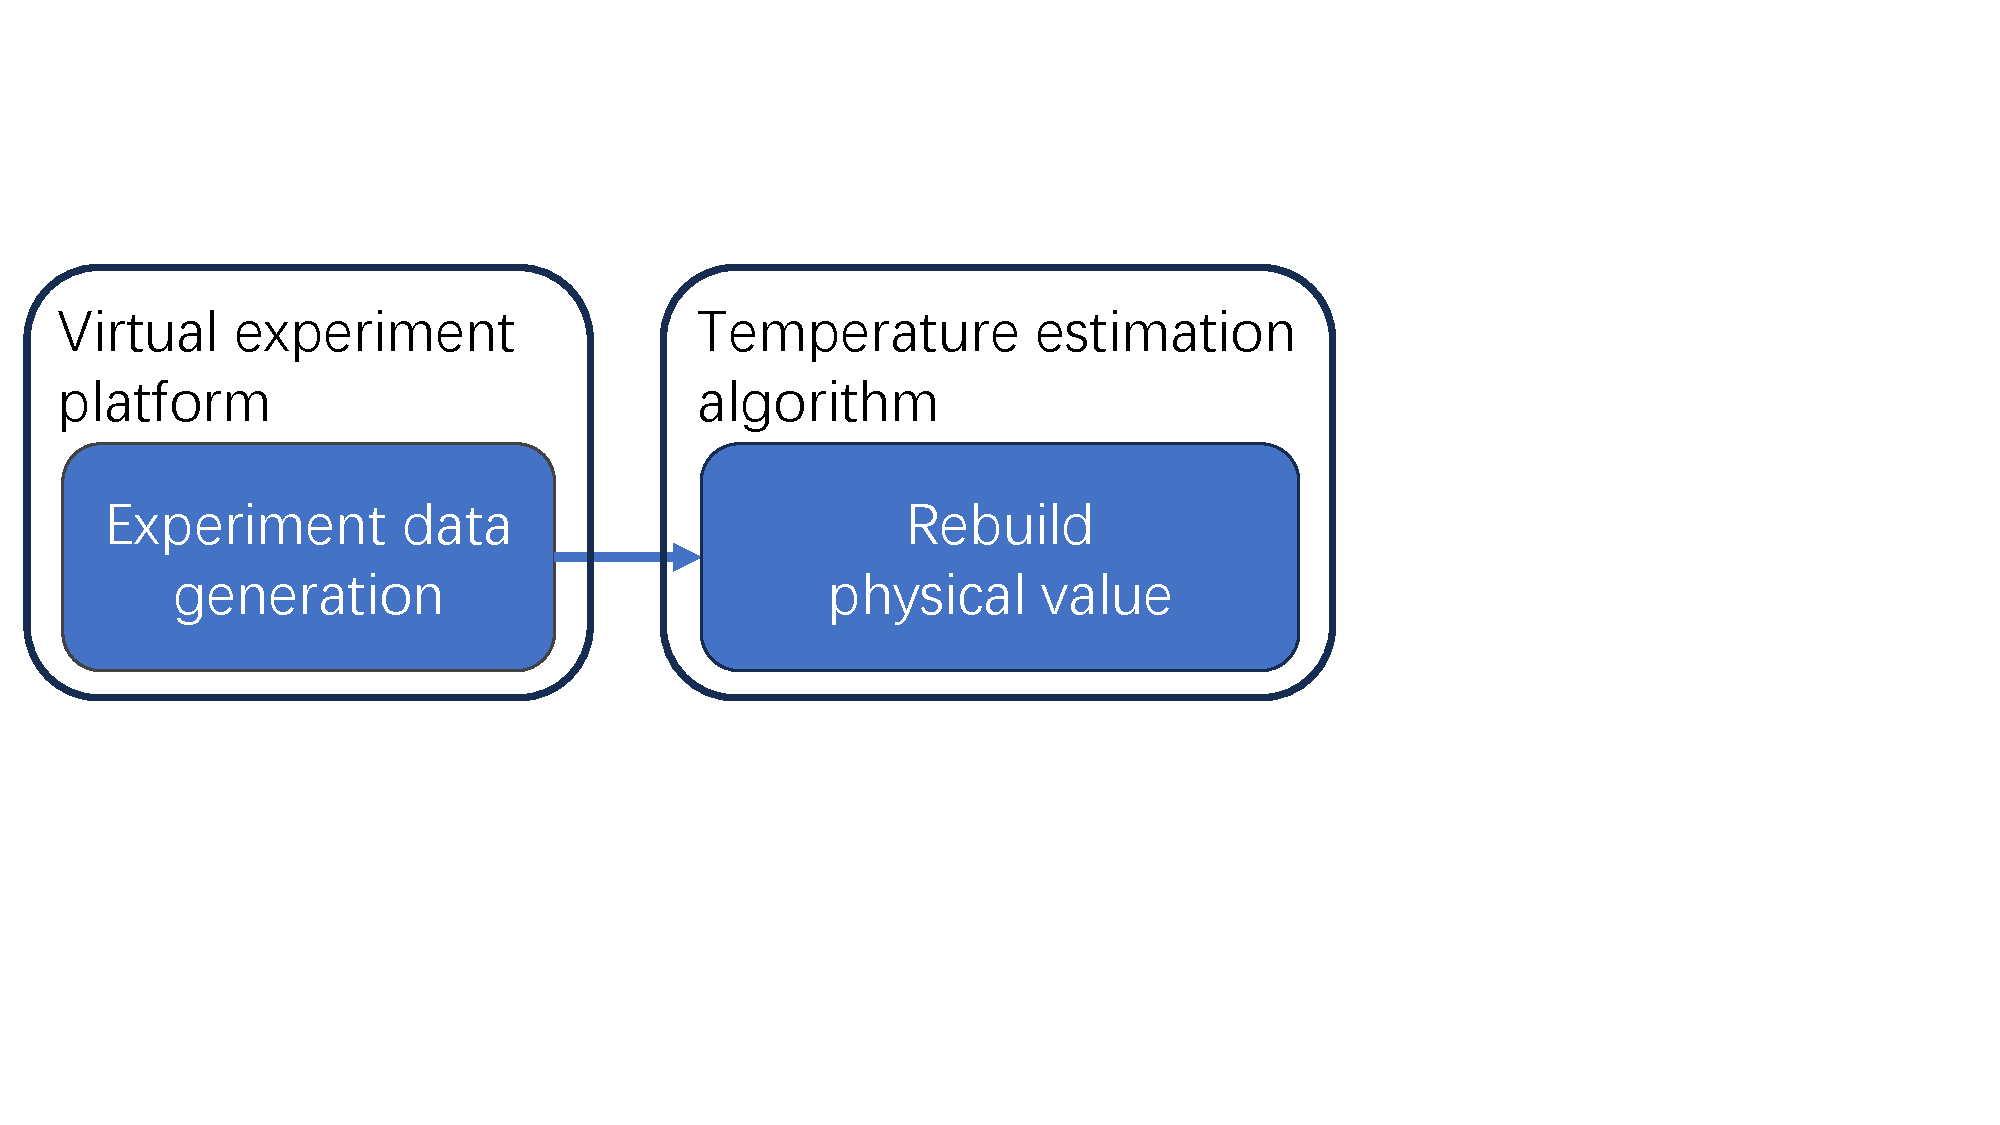
\includegraphics[width=0.6\textwidth]{figures/application_procedure_1.pdf}
    \caption{Complete procedure from data generation to model validation}
    \label{fig: application_procedure}
\end{figure}


Fig.\ref{fig: application_procedure} shows the procedure of the application.
Firstly, an experiment data set should be generated according to the parameters of the 
hypothetical material. Then, a temperature estimation algorithm is applied to 
estimate the temperature of the hypothetical material. Last, a validation procedure 
is used to check the accuracy and stability of the results of 
temperature estimation algorithm.


As mentioned in previous sections, these functions is implemented in three 
programmes. Namely virtual experiment platform, temperature estimation algorithm
and validation procedure. Similar to conventional experiment methods, these
steps are independent procedures, which means they do not interact with 
each other. 


Accordingly, this chapter will be divided into three sections, which describe 
the implementation and the parameter settings of the virtual experiment platform, 
temperature estimation algorithm and validation procedure.


\section{Experiment data generation}
As the first of the three steps mentioned above, it is crucial to generate 
accurate experimental data correctly. It affects the comparability of the 
virtual experimental platform with real experiments on the one hand, and 
the accuracy of the temperature estimation algorithm on the other. As a 
result, the virtual experimental platform should be able to perform 
calculations for as many hypothetical materials with different properties 
as possible.


In order to be able to obtain image similar to image from
real camera, the area that the virtual camera is able to capture is 
set to a 50*50 pixel picture. Fig.\ref{fig: camera} shows the image obtained 
from real experiment and virtual experiment platform. The major difference between 
these two images is the coloring. In real experiment, the raw image was saved 
as a .tiff file, which obtain the spectral intensity received by the specific 
channel. Then, the intensity is expressed as brightness of the pixel in the display of 
the image. This results in the experiment data that is not intuitive and 
requires specialised software to open these data.


As a result, there are a number of optimisations that have been applied 
in this virtual experiment platform. Firstly, the raw digital value 
of the received spectral intensity was saved in an .xlsx file, which 
simplifies the reading of the data as well as the conversion. In 
addition, a .jpg image of each channel similar to the real experiment data is also 
saved. Different from the real experiment data, colours are used here to 
indicate the value of the spectral intensity. This improves the 
readability of the experiment data.


\begin{figure}[htbp]
    \centering
    \begin{subfigure}{0.45\textwidth}
        \centering
        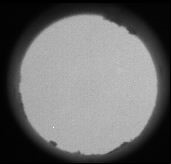
\includegraphics[height=5cm]{figures/real_camera_1075.JPG}
        \caption{Real experiment data  (channel 1)}
        \label{fig: real_camera}
    \end{subfigure}
    % \hfill
    \begin{subfigure}{0.45\textwidth}
        \centering
        
\includegraphics[height=5cm]{figures/virtual_camera_1098.jpg}
        \caption{Virtual experiment data (channel 1)}
        \label{fig: virtual_camera}
    \end{subfigure}
    \caption{Comparison between real experiment data at $1300K$ (a)
    and virtual experiment data at $1098K$ (b)
    }
    \label{fig: camera}
\end{figure}


Thus, the observation area is obtained by initialization of the the virtual 
experiment platform. Temperature field, emissivity model of the hypothetical 
material and the integration method are the parameters to be defined as the next
step.


\subsection{Temperature field}%
As mentioned in previous sections, temperature is one of the most important parameters 
in the virtual experiment platform. In order to obtain results similar to real 
experiments, a temperature field exists in the observation area. For the purpose of 
simplifying the calculation process, this temperature field consists of two main 
regions, a background region at the edge of the observation area, 
where the temperature is uniformly set to 1000K, and an internal high temperature 
region, where the temperature follows a predefined distribution.


\begin{figure}[htbp]
    \centering
    \begin{subfigure}{0.08\textwidth}
        \centering
        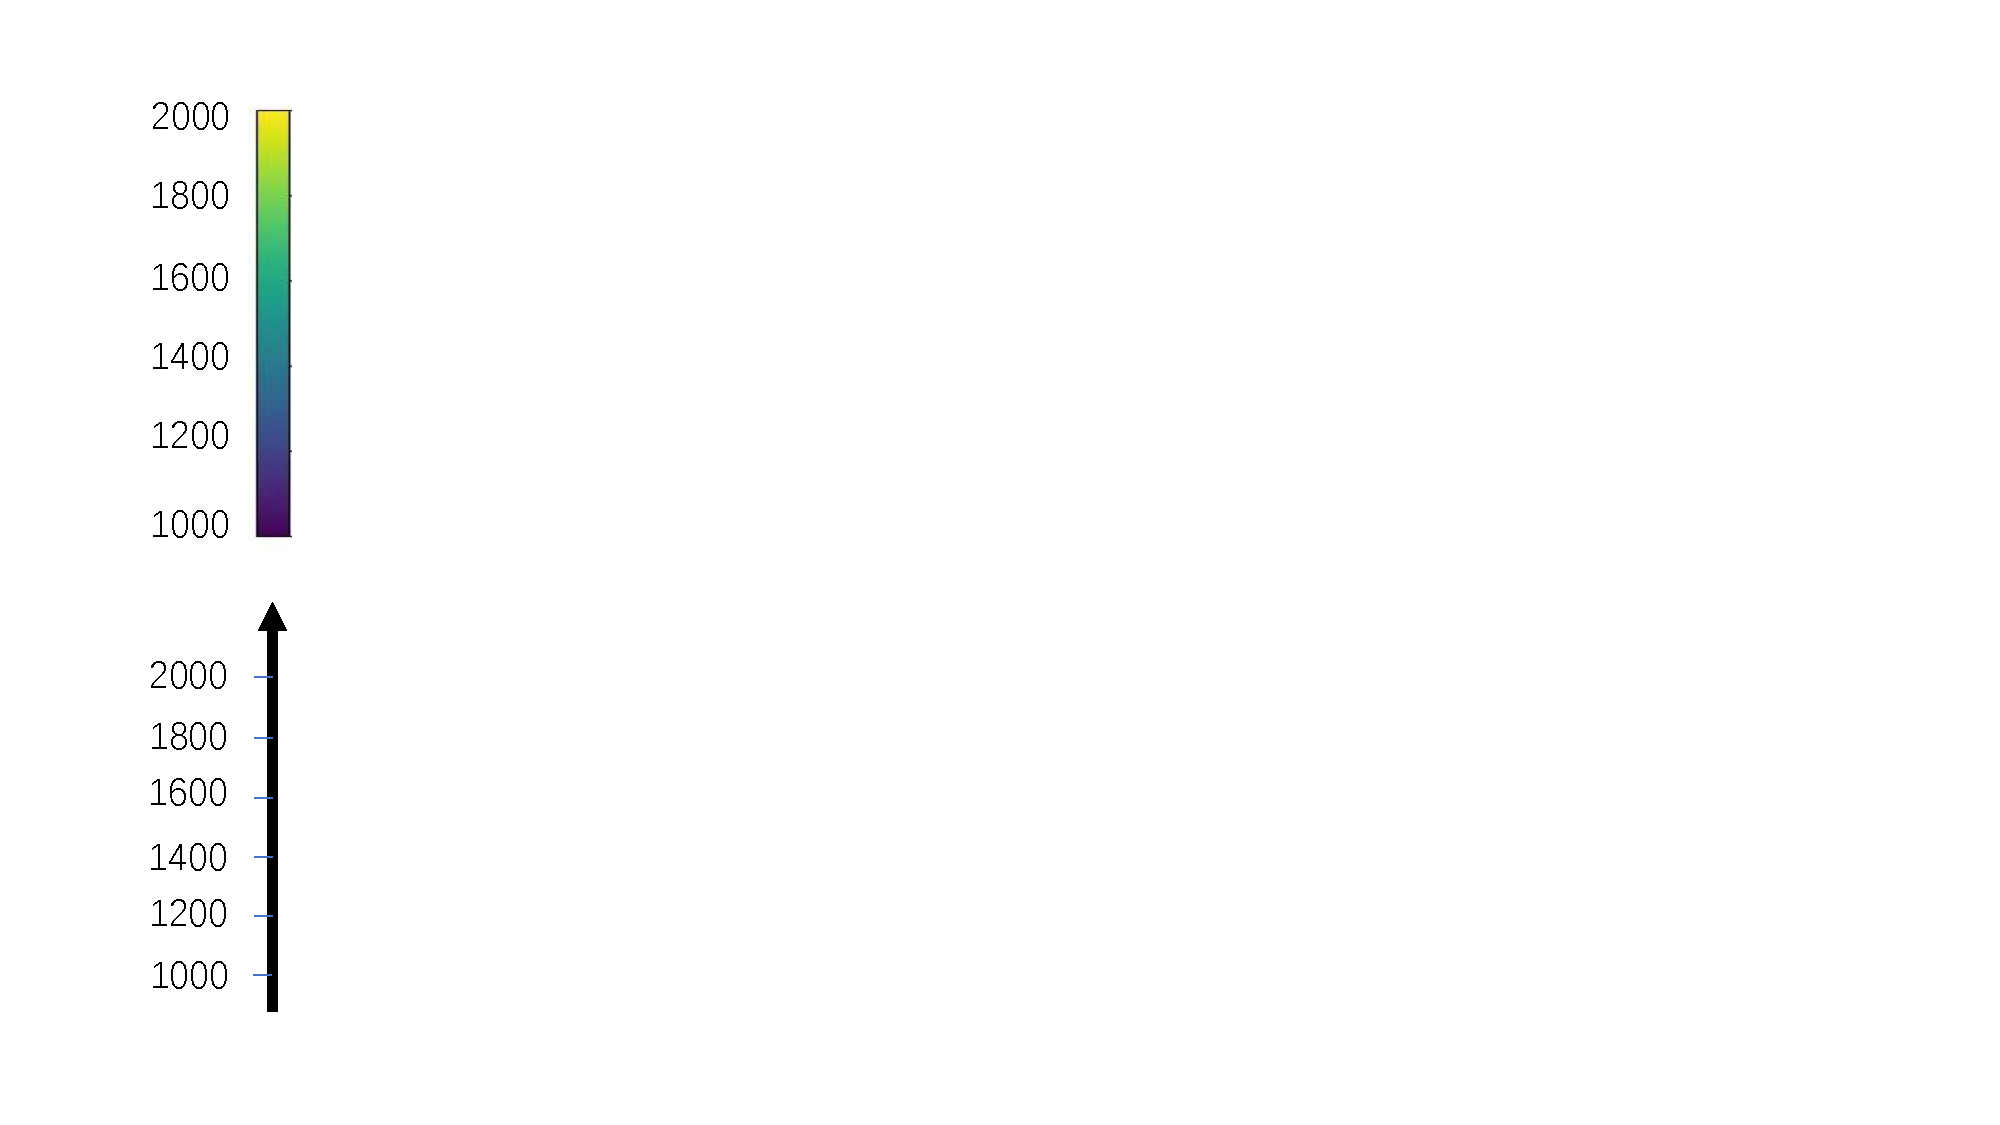
\includegraphics[height=9cm]{figures/temp_distribution_colorbar.pdf}
        \caption*{}        
    \end{subfigure}
    \begin{subfigure}{0.3\textwidth}
        \centering
        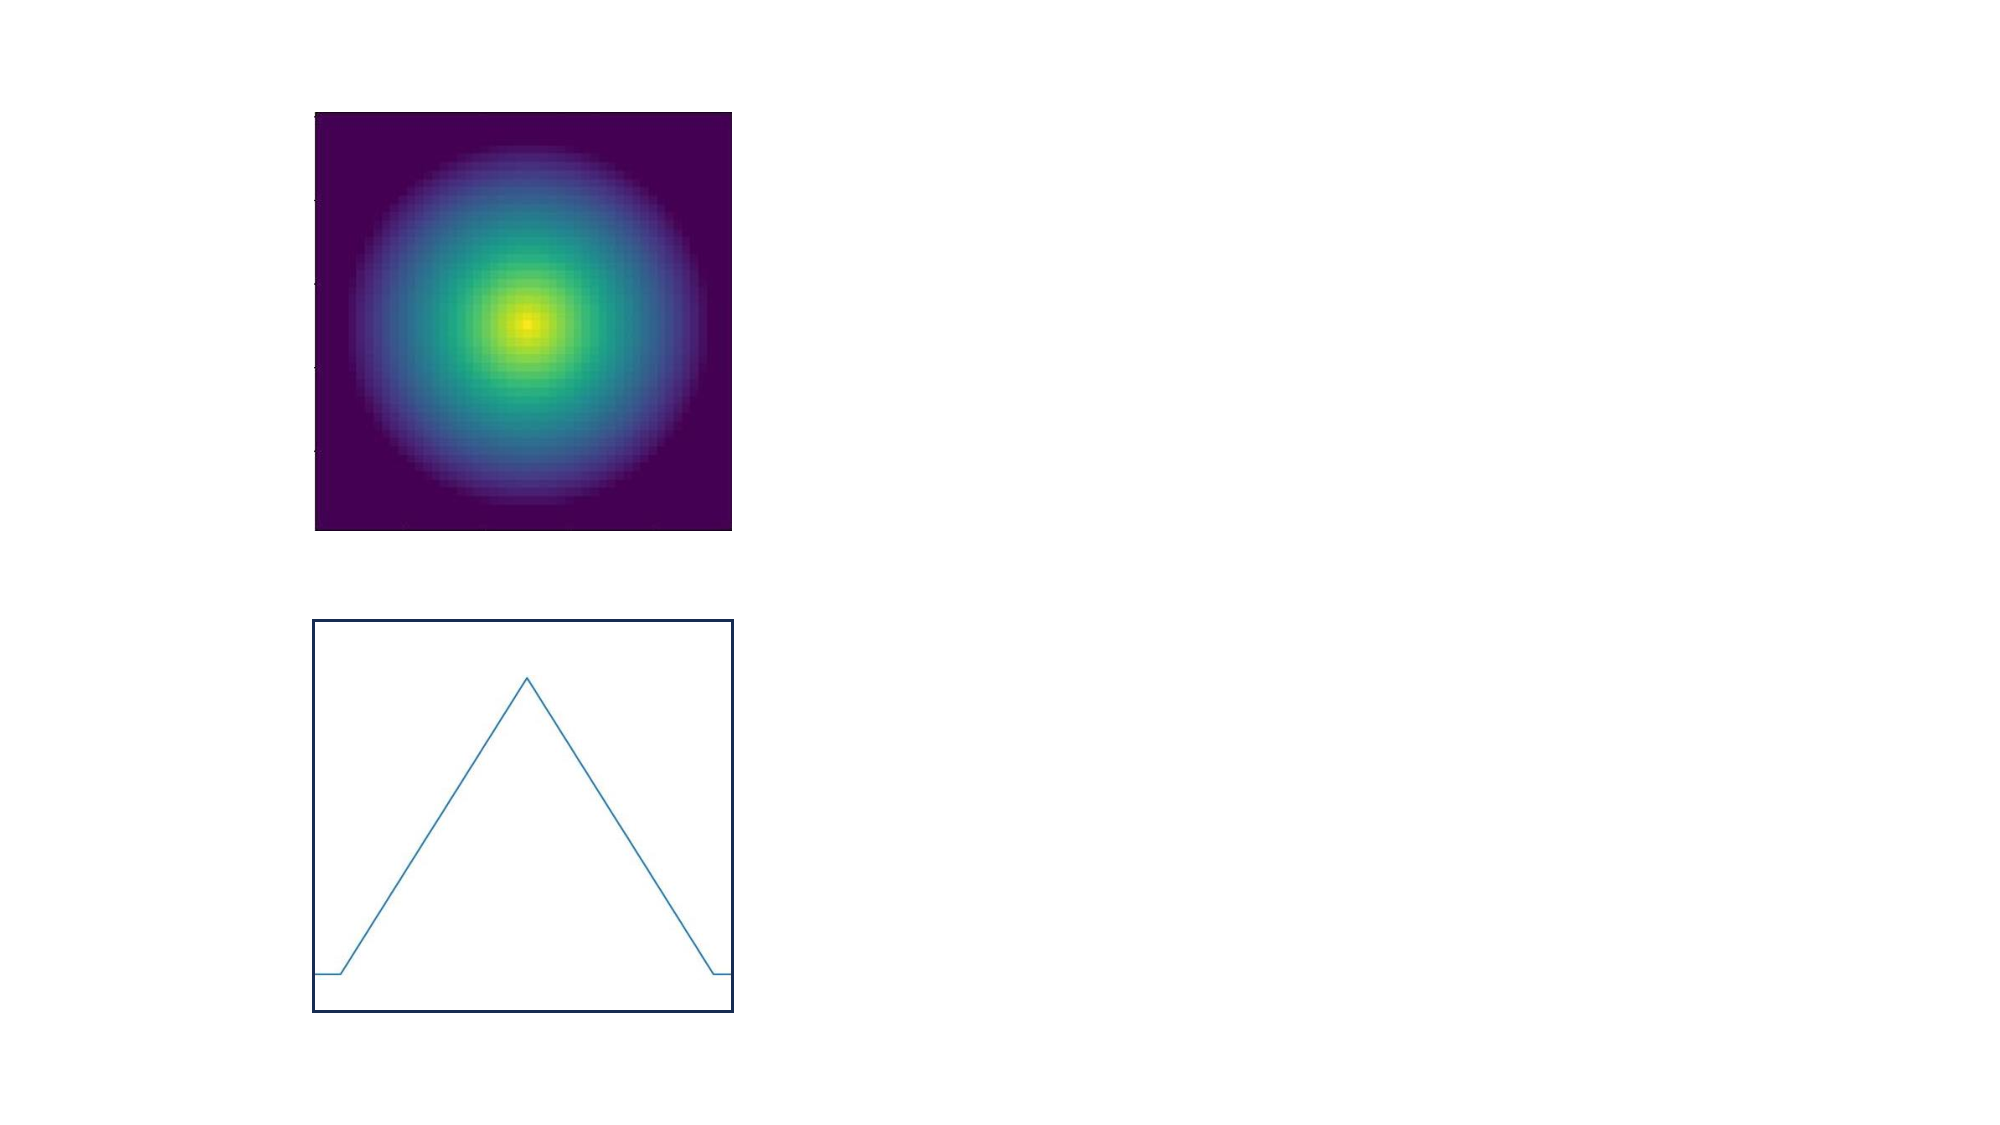
\includegraphics[height=9cm]{figures/temp_distribution_a.pdf}
        \caption{Linear}
        \label{fig: linear_distribution}        
    \end{subfigure}
    \begin{subfigure}{0.3\textwidth}
        \centering
        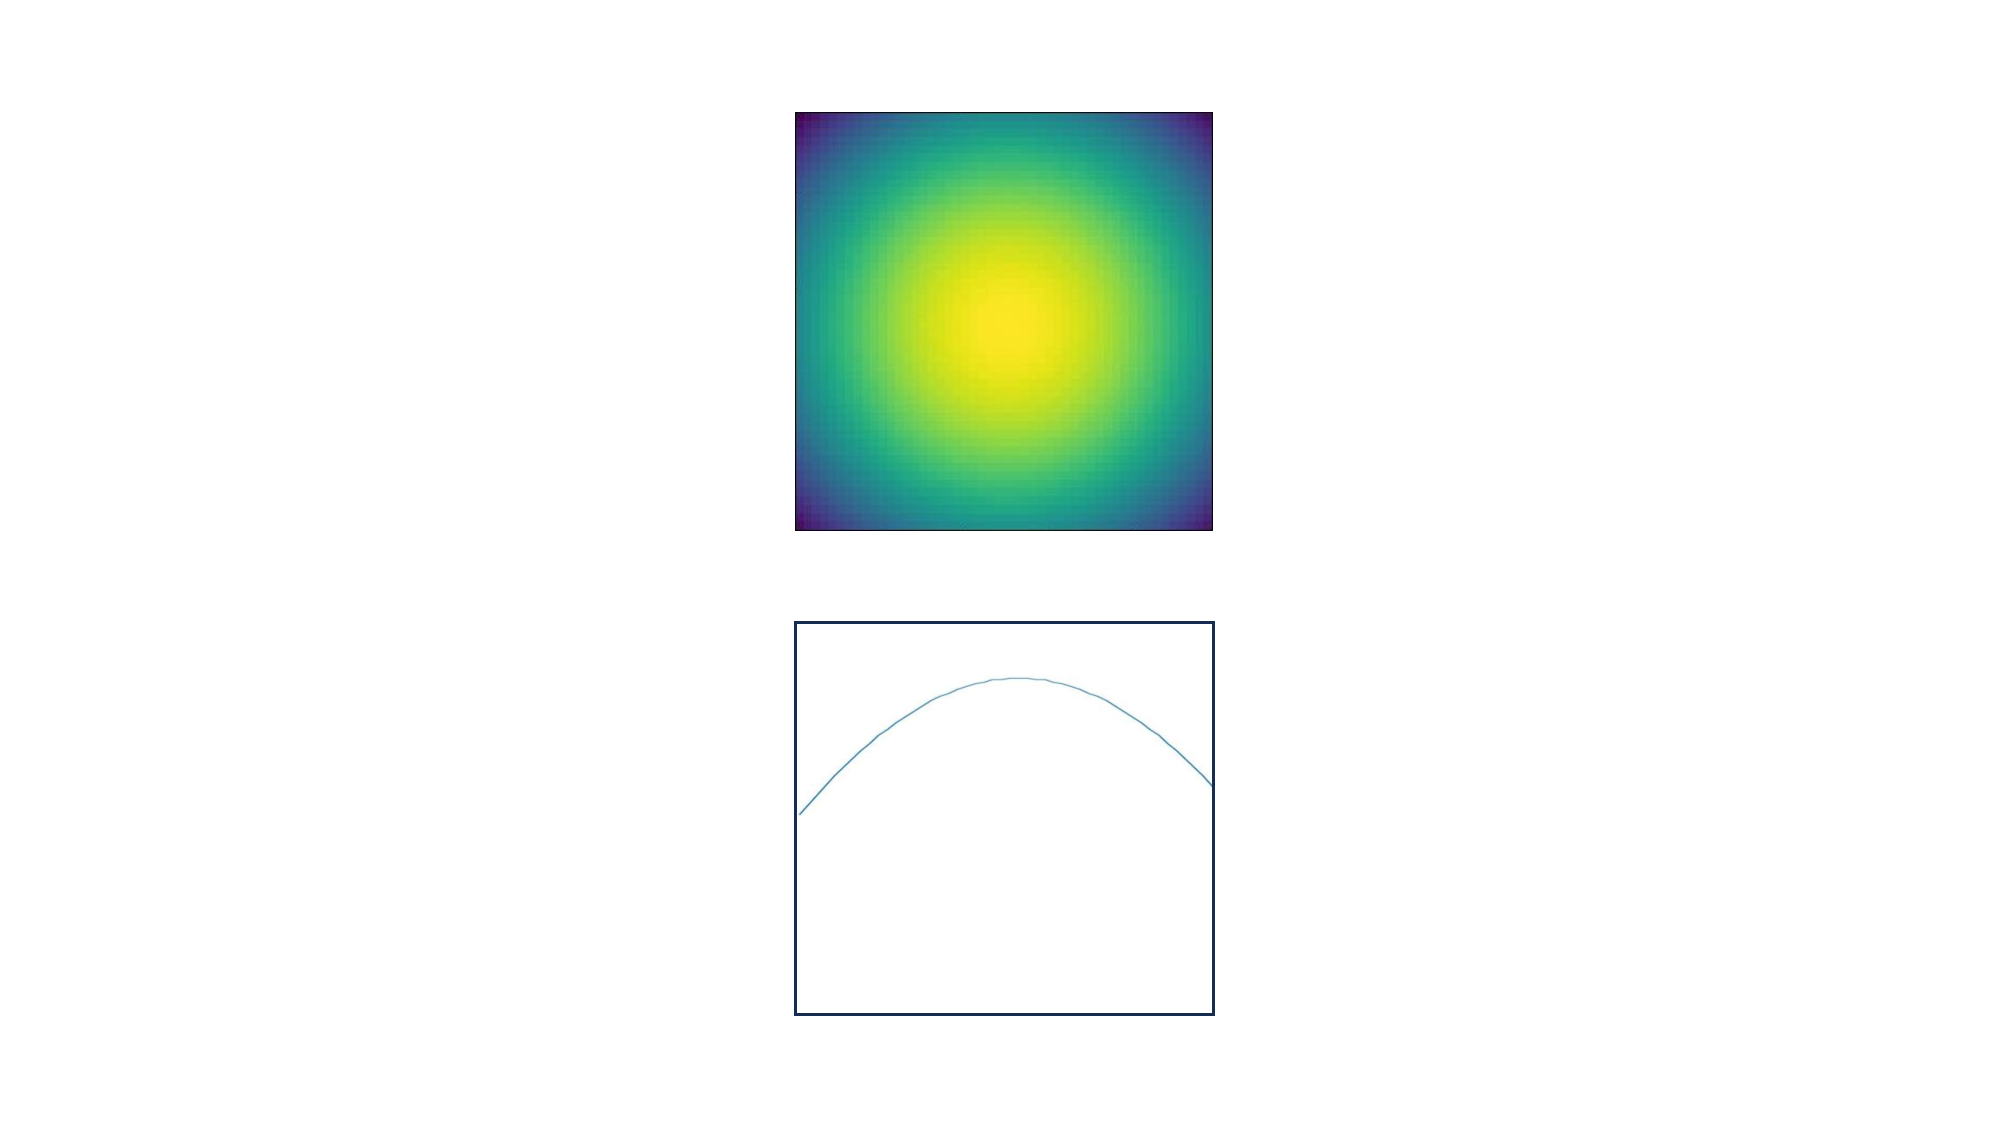
\includegraphics[height=9cm]{figures/temp_distribution_b.pdf}
        \caption{Gaussian}
        \label{fig: gaussian_distribution}        
    \end{subfigure}
    \begin{subfigure}{0.3\textwidth}
        \centering
        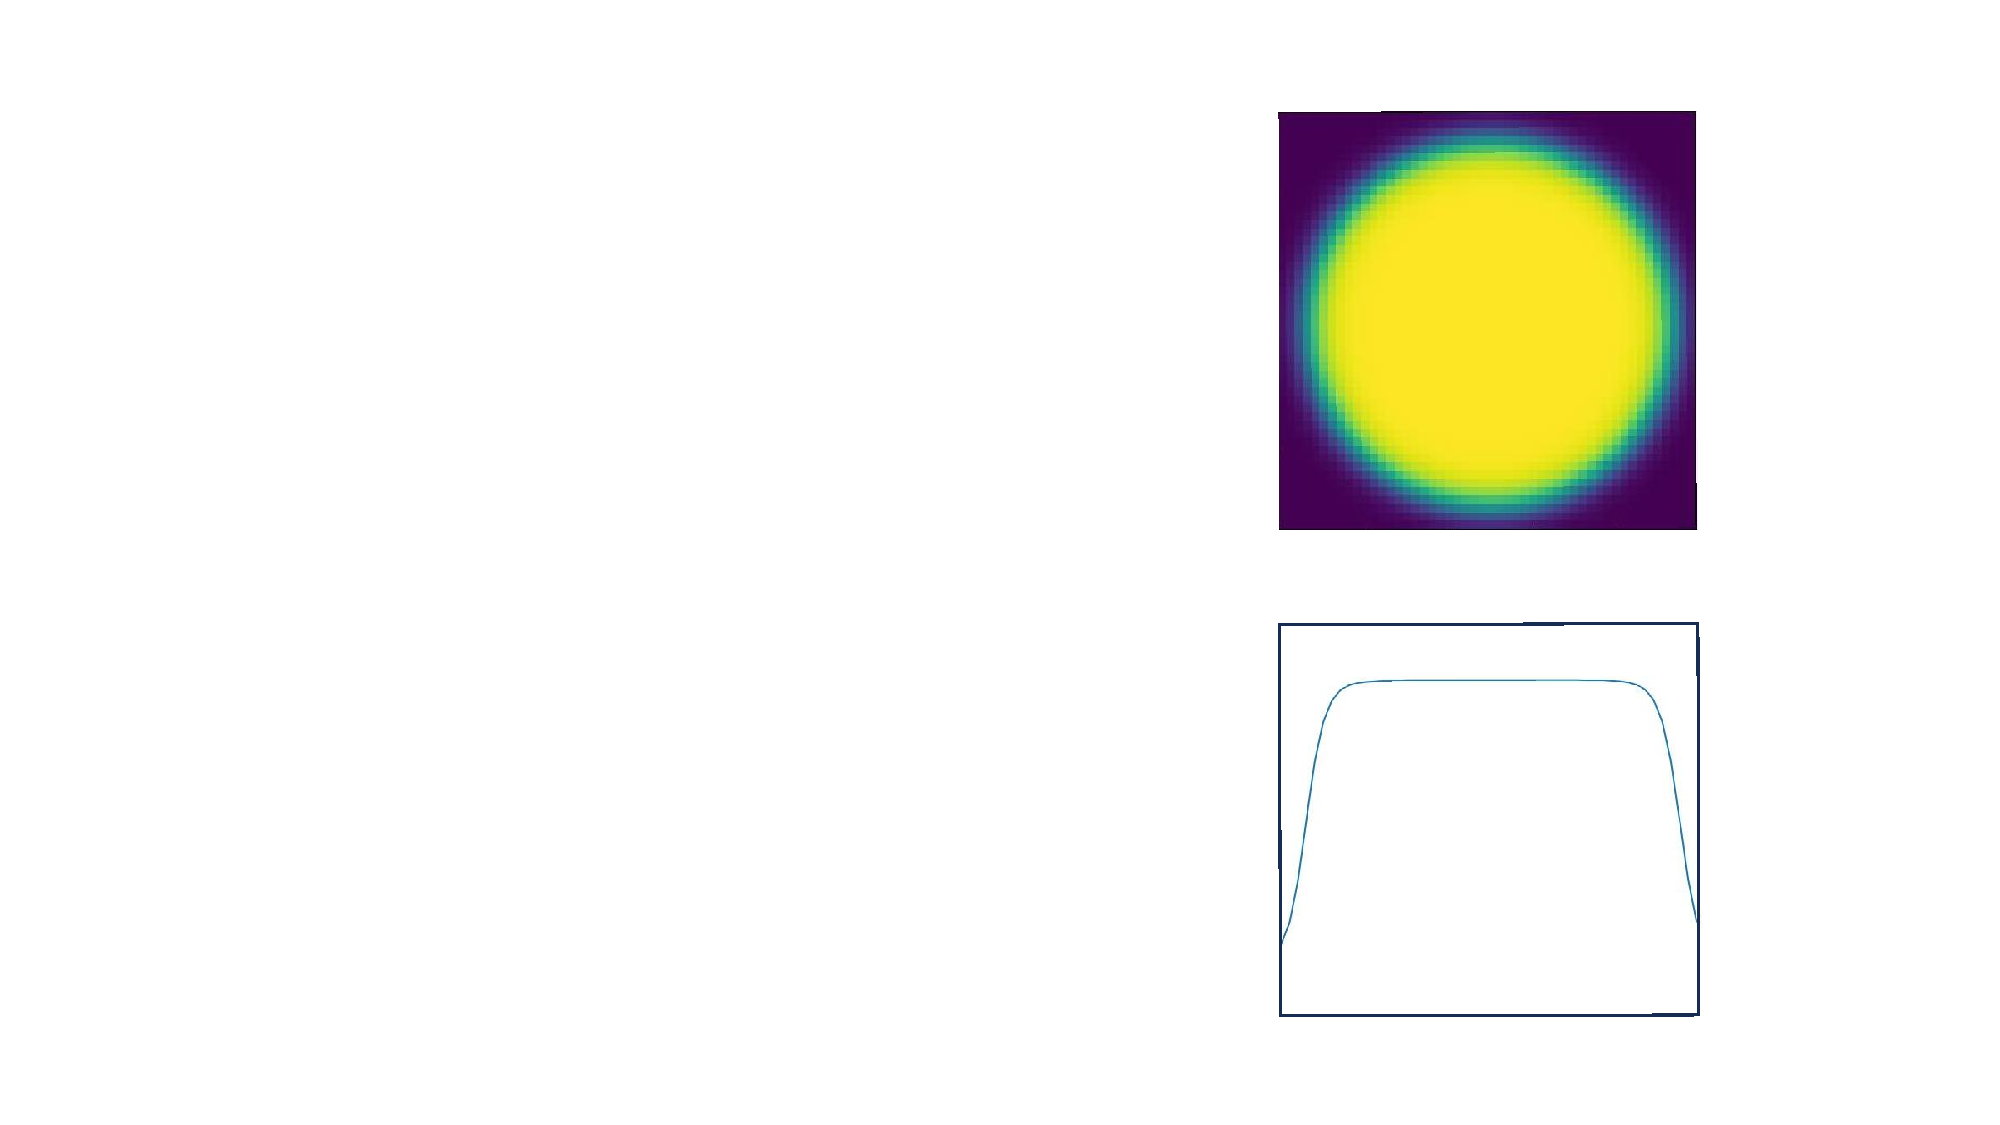
\includegraphics[height=9cm]{figures/temp_distribution_c.pdf}
        \caption{Sigmoid}
        \label{fig: sigmoid_distribution}        
    \end{subfigure}
    \caption{Temperature field of 3 different temperature distribution and the 
    temperature profile in the middle line of the observation area. (\subref{fig: linear_distribution}): 
    Linear distribution. (\subref{fig: gaussian_distribution}): Gaussian distribution. 
    (\subref{fig: sigmoid_distribution}): sigmoid distribution}
    \label{fig: temperature_profile}
\end{figure}


Fig.\ref{fig: temperature_profile} shows three different temperature distribution 
which are able to be generated by the virtual experiment platform. Namely linear 
distribution, gaussian distribution and sigmoid distribution. In order to simplify 
the visualization process, all temperature fields are generated based on the center 
point of the observation area. As the temperature of each point is calculated 
based on the normalized distance $d_{rel}$ or absolute distance ${d_{abs}}$ to the center point of the observation area.


Linear distribution means that the temperature increases linearly from the back ground 
area to the center point of the observation area. The details can be found in 
Eq.\ref{eq: linear_distribution}. This distribution has the potential to 
demonstrate the spectral radiation behavior of the hypothetical material in 
different temperature. 


\begin{equation}
    t = t_{center} + (t_{background} - t_{center}) \cdot d_{rel}
    \label{eq: linear_distribution}
\end{equation}


Gaussian distribution is also called normal distribution. In this distribution 
type, the temperature field in observation area obeys gaussian distribution described 
in Eq.\ref{eq: gaussian_distribution}. With the temperature of the center 
point in observation area equals the defined center temperature. Due to energy input 
of the system and heat transfer in metal powder, this temperature distribution 
is more likely to simulate the real situation in experiment.

\begin{equation}
    t = t_{center} + (t_{background} - t_{center}) \cdot \exp {\left(-\frac{d_{abs}}{2 \cdot \sigma^2}\right)}
    \label{eq: gaussian_distribution}
\end{equation}


Different to the temperature field mentioned before, the temperature in the center region 
of observation area remains constant. The mathematical expression can be found in 
Eq.\ref{eq: sigmoid_distribution}:

\begin{equation}
    t = t_{center} + (t_{background} - t_{center}) \cdot \sigmoid\left( \left(\frac{d_{abs}^2}{r_{set}^2} + 1\right)\cdot 1000\right)
    \label{eq: sigmoid_distribution}
\end{equation}


With sigmoid function can be found in Eq.\ref{eq: sigmoid_function}:

\begin{equation}
    \sigmoid(x) = \left(1 + \exp\left(-\frac{x}{100}\right)\right)
    \label{eq: sigmoid_function}
\end{equation}


Sigmoid function gaves the opportunity to perform the temperature estimation algorithm 
in a stable temperature. Thus, the potential to investigate the consistency of the 
temperature estimation algorithm and performance of the noise cancellation program is 
given. 


\subsection{Emissivity model}%
Obtaining temperature field of the hypothetical material, an emissivity model 
is required to calculate the physical value of spectral radiation intensity 
emitted from the hypothetical material.


\begin{figure}[htbp]
    \centering
    \begin{subfigure}{0.3\linewidth}
      \centering
      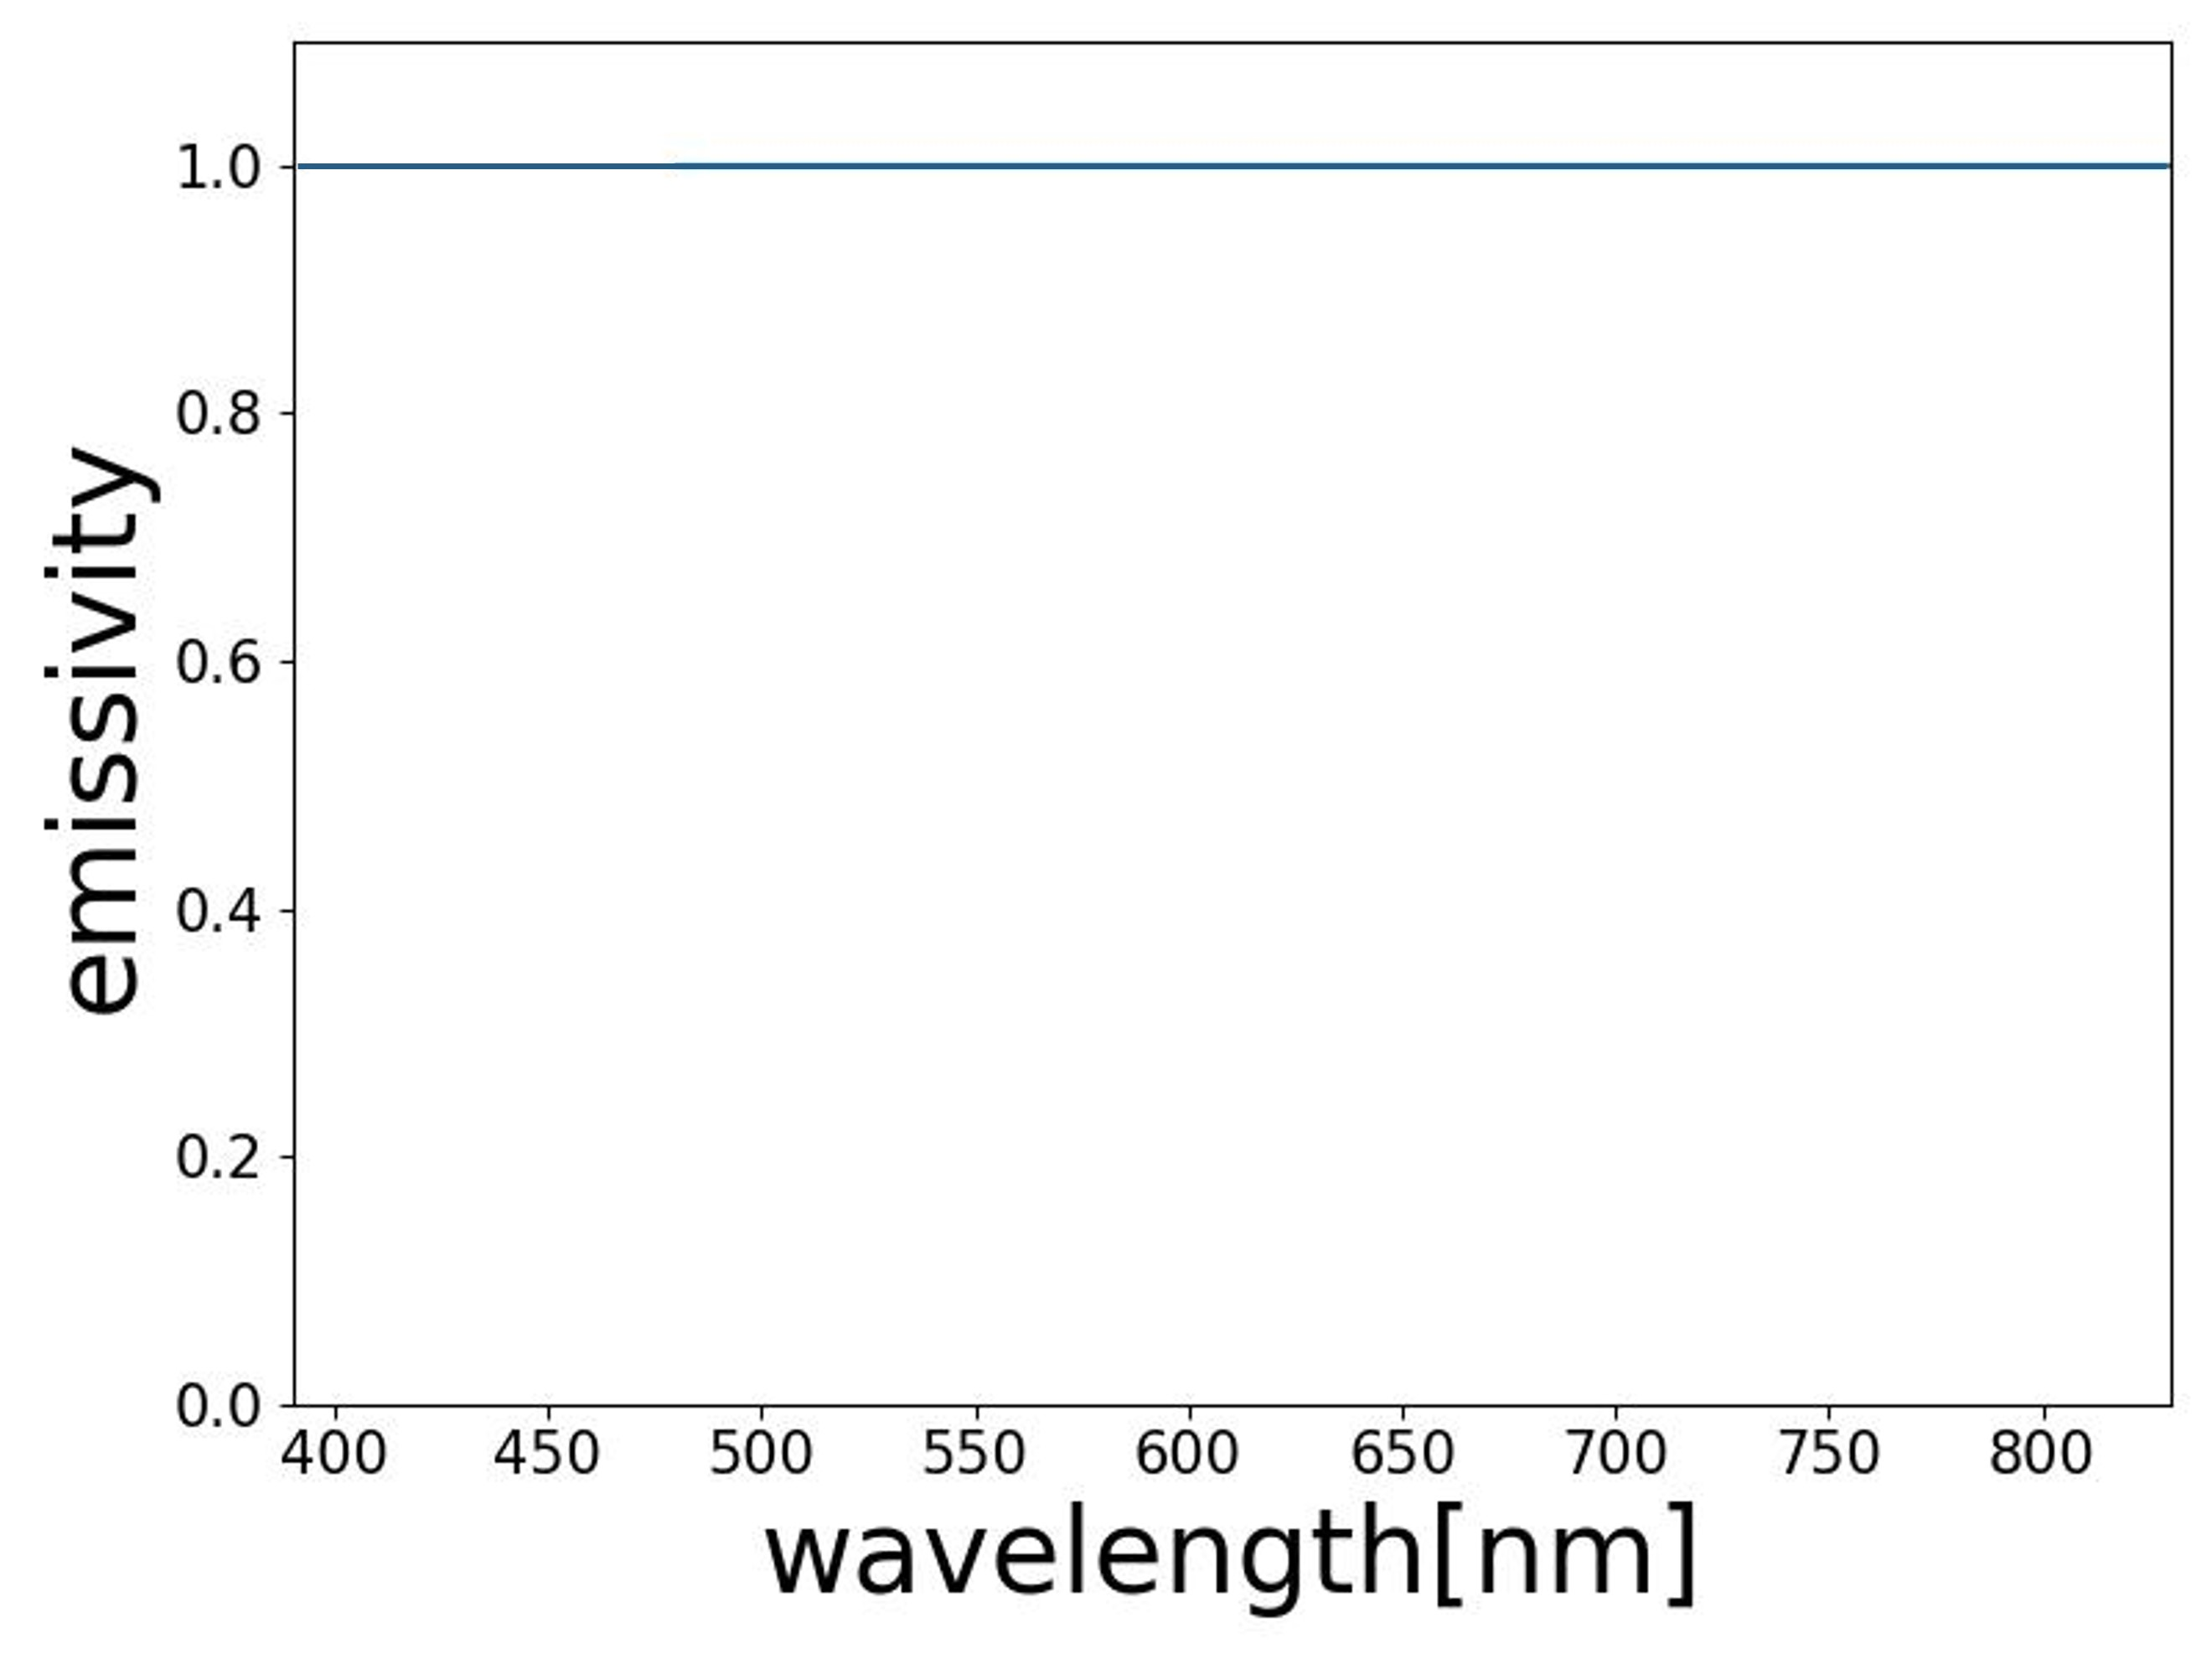
\includegraphics[width=\linewidth]{figures/emissivity_0.jpg}
      \caption{Black body model}
      \label{fig: emi_0}
    \end{subfigure}
    \hfill
    \begin{subfigure}{0.3\linewidth}
      \centering
      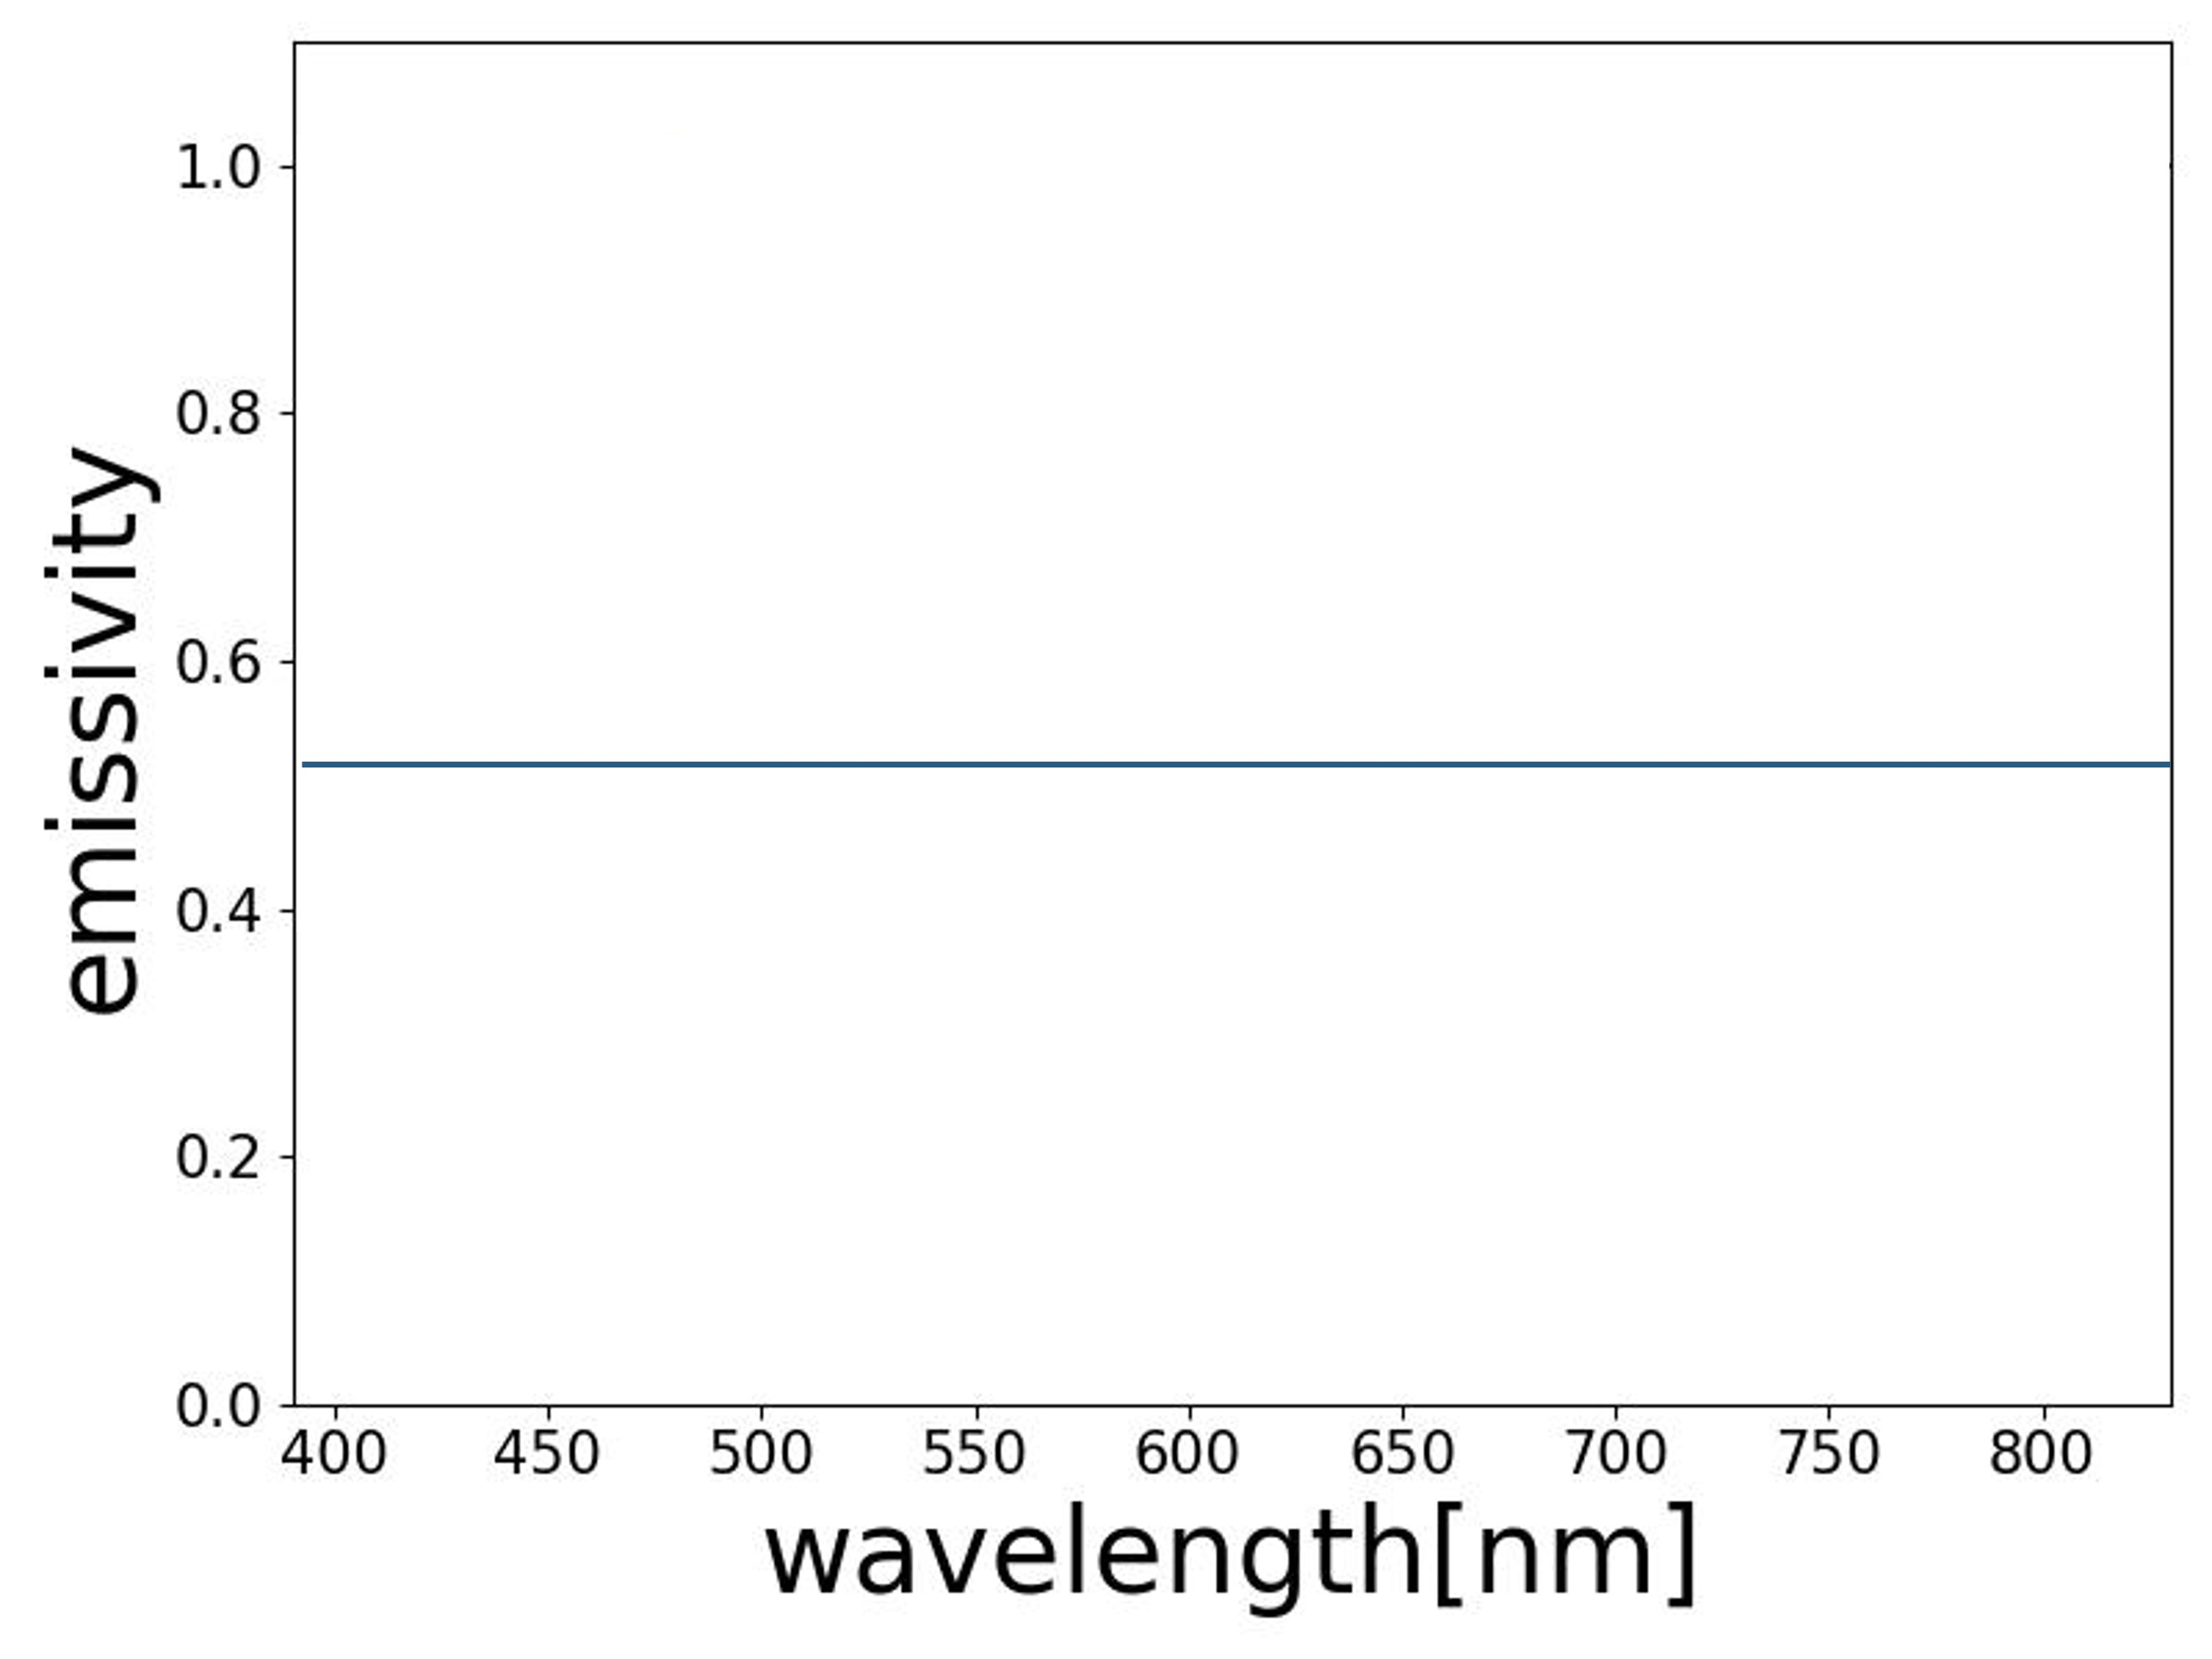
\includegraphics[width=\linewidth]{figures/emissivity_1.jpg}
      \caption{Gray body model}
      \label{fig: emi_1}
    \end{subfigure}
    \hfill
    \begin{subfigure}{0.3\linewidth}
      \centering
      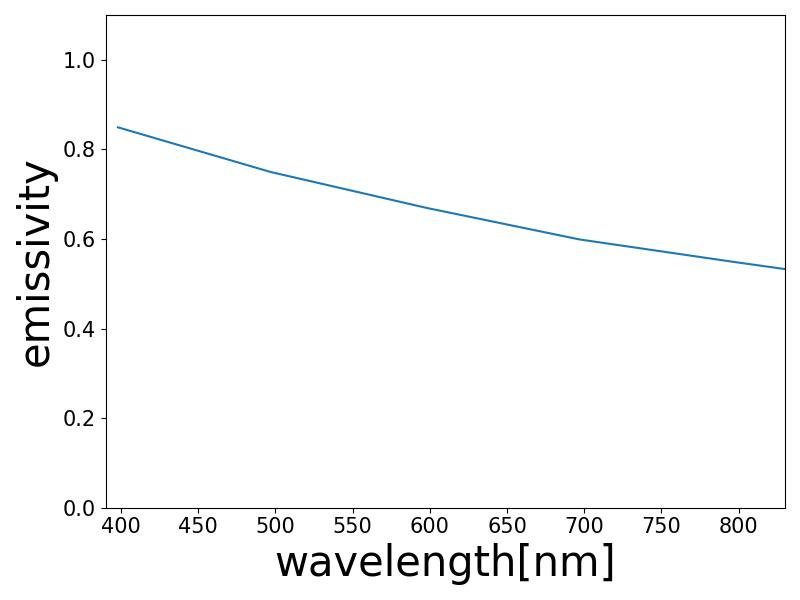
\includegraphics[width=\linewidth]{figures/emissivity_21.jpg}
      \caption{Model 1}
      \label{fig: emi_21}
    \end{subfigure}
    
    \medskip
    
    \begin{subfigure}{0.3\linewidth}
      \centering
      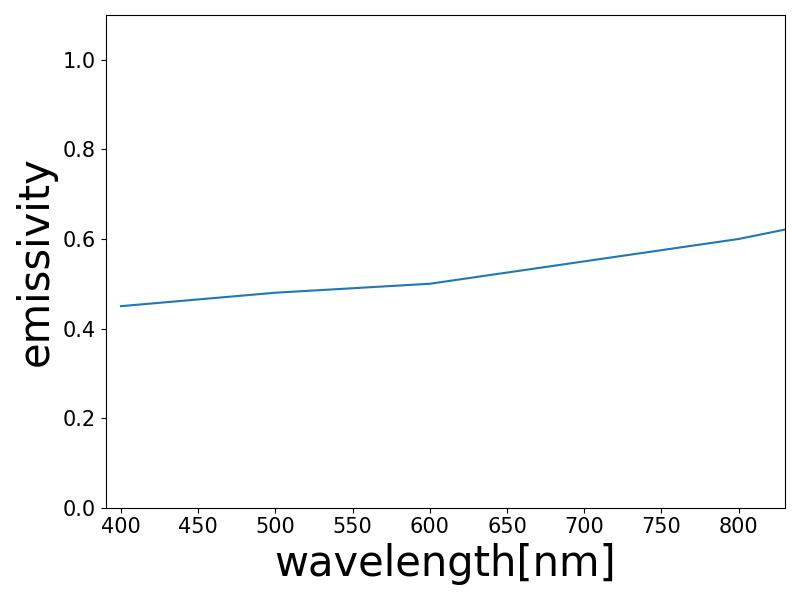
\includegraphics[width=\linewidth]{figures/emissivity_22.jpg}
      \caption{Model 2}
      \label{fig: emi_22}
    \end{subfigure}
    \hfill
    \begin{subfigure}{0.3\linewidth}
      \centering
      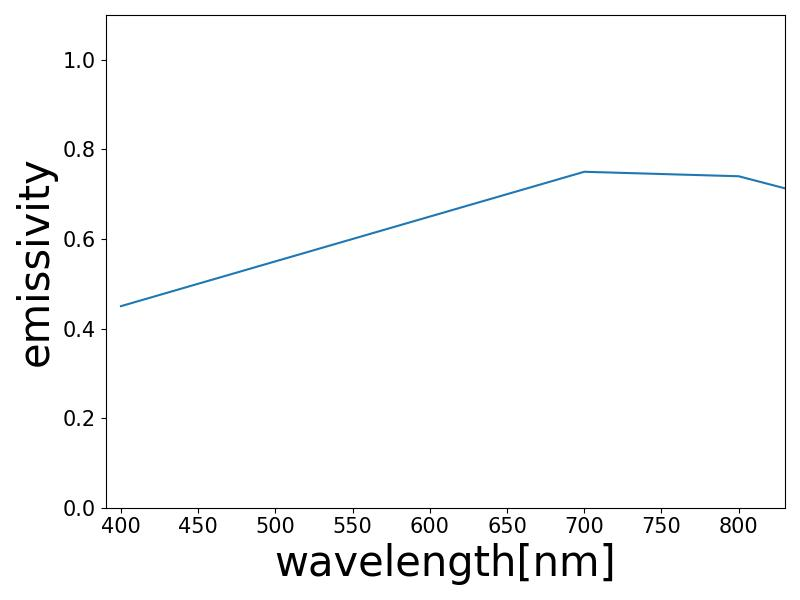
\includegraphics[width=\linewidth]{figures/emissivity_23.jpg}
      \caption{Model 3}
      \label{fig: emi_23}
    \end{subfigure}
    \hfill
    \begin{subfigure}{0.3\linewidth}
      \centering
      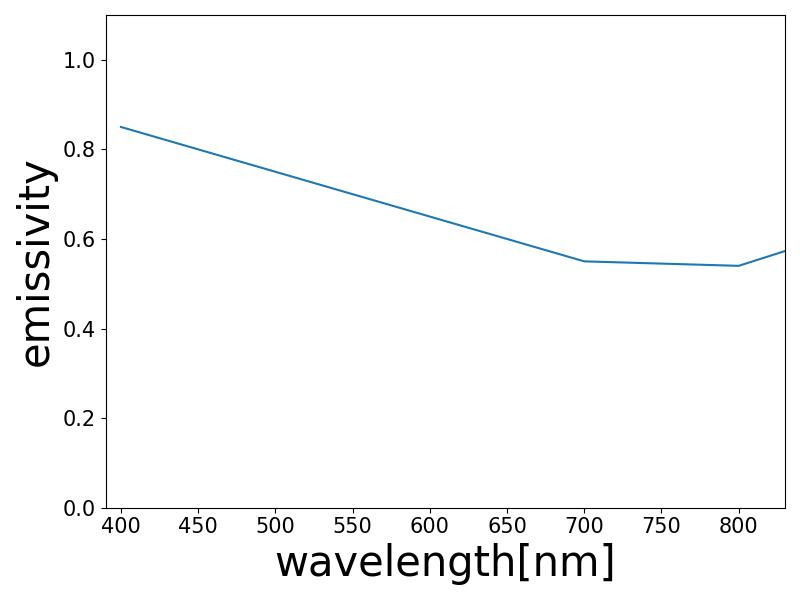
\includegraphics[width=\linewidth]{figures/emissivity_24.jpg}
      \caption{Model 4}
      \label{fig: emi_24}
    \end{subfigure}
    
    \medskip
    
    \begin{subfigure}{0.3\linewidth}
      \centering
      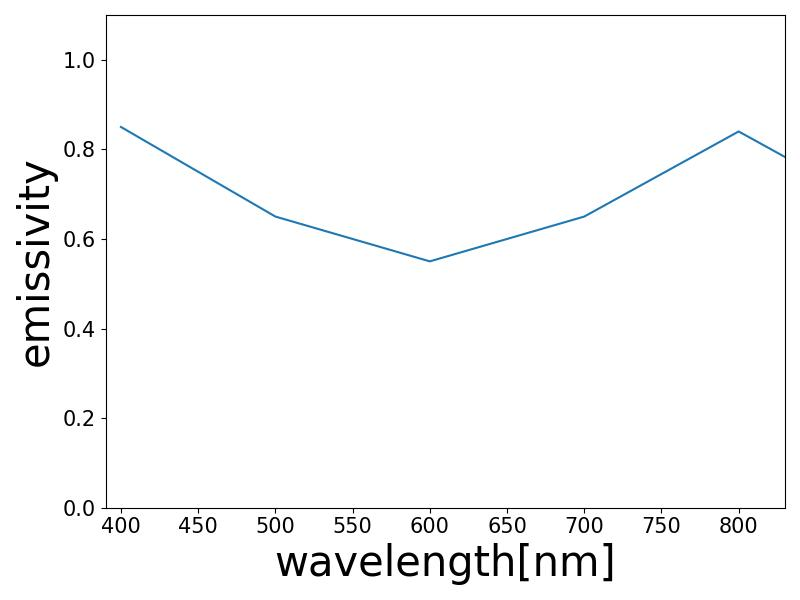
\includegraphics[width=\linewidth]{figures/emissivity_25.jpg}
      \caption{Model 5}
      \label{fig: emi_25}
    \end{subfigure}
    \hfill
    \begin{subfigure}{0.3\linewidth}
      \centering
      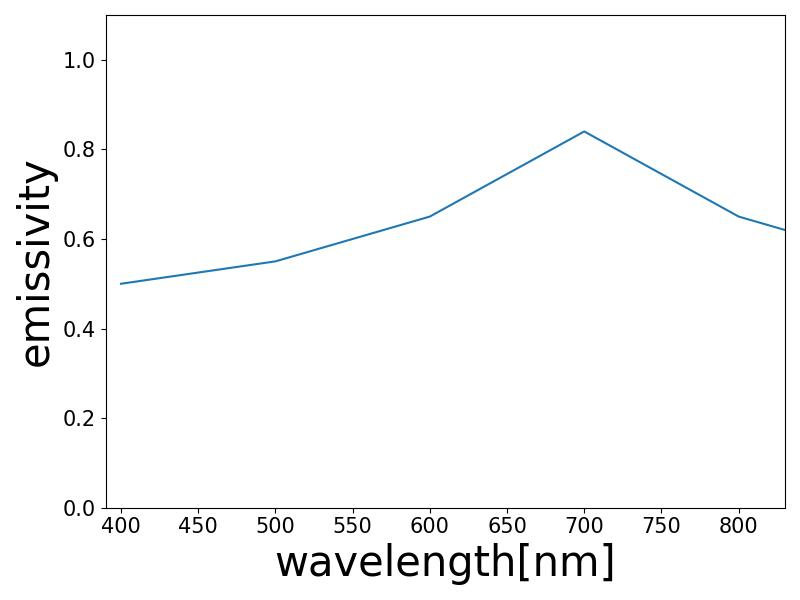
\includegraphics[width=\linewidth]{figures/emissivity_26.jpg}
      \caption{Model 6}
      \label{fig: emi_26}
    \end{subfigure}
    \hfill
    \begin{subfigure}{0.3\linewidth}
      \centering
      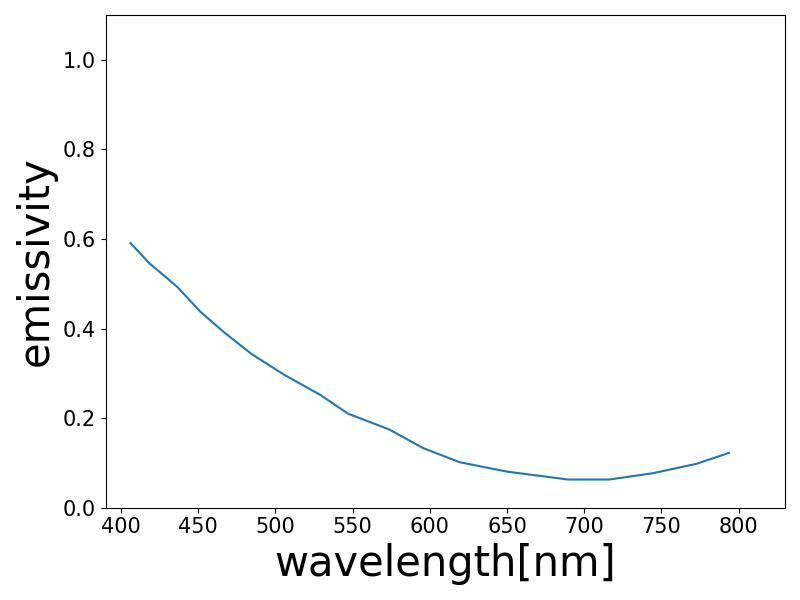
\includegraphics[width=\linewidth]{figures/emissivity_31.jpg}
      \caption{Model 7}
      \label{fig: emi_31}
    \end{subfigure}
    
    \medskip
    
    \begin{subfigure}{0.3\linewidth}
      \centering
      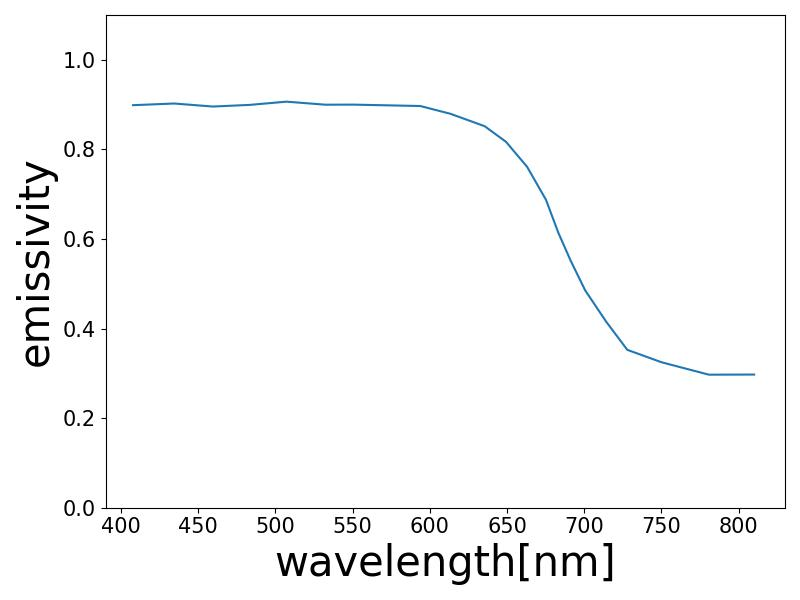
\includegraphics[width=\linewidth]{figures/emissivity_32.jpg}
      \caption{Model 8}
      \label{fig: emi_32}
    \end{subfigure}
    \hfill
    \begin{subfigure}{0.3\linewidth}
      \centering
      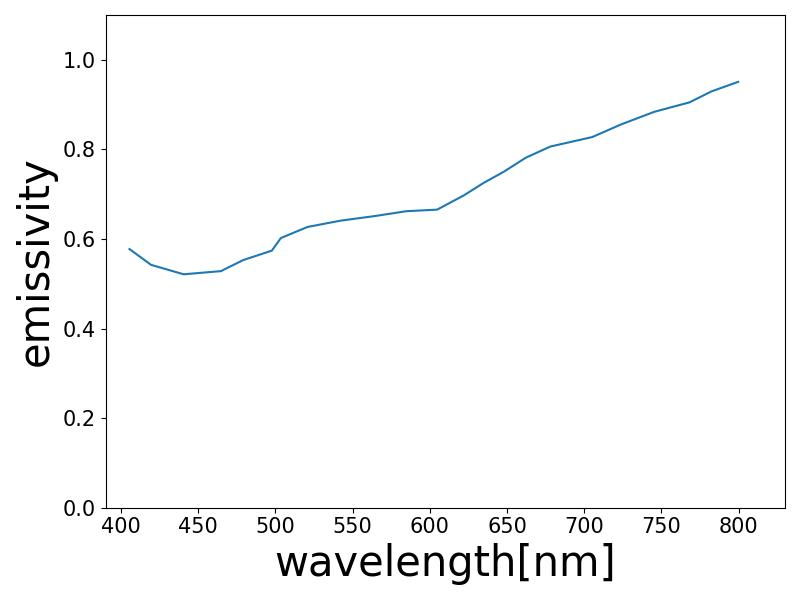
\includegraphics[width=\linewidth]{figures/emissivity_33.jpg}
      \caption{Model 9}
      \label{fig: emi_33}
    \end{subfigure}
    \hfill
    \begin{subfigure}{0.3\linewidth}
      \centering
      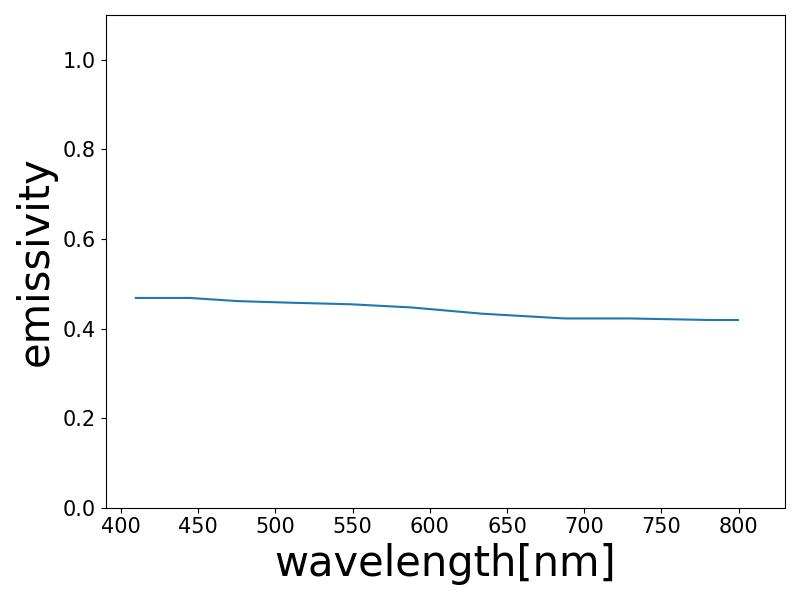
\includegraphics[width=\linewidth]{figures/emissivity_34.jpg}
      \caption{Model 10}
      \label{fig: emi_34}
    \end{subfigure}
    
    \caption{Raw emissivity data used in virtual experiment platform. (\subref{fig: emi_0}), 
    (\subref{fig: emi_1}) are black body and gray body; (\subref{fig: emi_21}) - (\subref{fig: emi_26})
    are hypothetical materials\cite{Wang.2021b}; (\subref{fig: emi_31}) - 
    (\subref{fig: emi_34}) are real materials\cite{Taunay.2020b}.}
    \label{fig: emi_model}
\end{figure}


Since the emissivity of metal powder is wavelength ($\lambda$) and temperature 
($T$) relevant, the emissivity model in this virtual experiment platform is 
formed based on the Eq.\ref{eq: emissivity}. 


\begin{equation}
  \label{eq: emissivity}
  \varepsilon(\lambda, T) = \varepsilon _{raw}(\lambda) \cdot K_T(T)
\end{equation}


The raw emissivity data $\varepsilon_{raw}(\lambda)$ in Fig.\ref{fig: emi_model}
are obtained by Wang et al.\cite{Wang.2021b} and Taunay et 
al.\cite{Taunay.2020b}. These data sets could be used to simulate the 
radiation behavior of various hypothetical materials.


After obtaining the raw data on the relationship between emissivity 
and wavelength, the dependence of emissivity on temperature is characterised
as a temperature factor $K_T(T)$ in Eq.\ref{eq: k_t}.

\begin{equation}
  \label{eq: k_t}
  K_T(T)=\begin{cases}
    1 - T_{ref} \cdot 0.2 &   T<T_{melt}\\
    \left(1 - T_{ref} \cdot 0.2 \right) \cdot 0.1 &  T\geq T_{melt}
  \end{cases}
\end{equation}


With 

\begin{equation}
  \label{eq: t_ref}
  T_{ref}=\frac{T - T_{lb}}{T_{ub} - T_{lb}}
\end{equation}


This temperature factor describes the tendency 
of emissivity to decrease with increasing temperature between $T_{lb}$ and $T_{ub}$, 
on the other hand, it also describes the change of emissivity due to the 
phase change of the hypothetical material that occurs at melting 
temperature $T_{melt}$.

\begin{figure}[htbp]
  \centering
  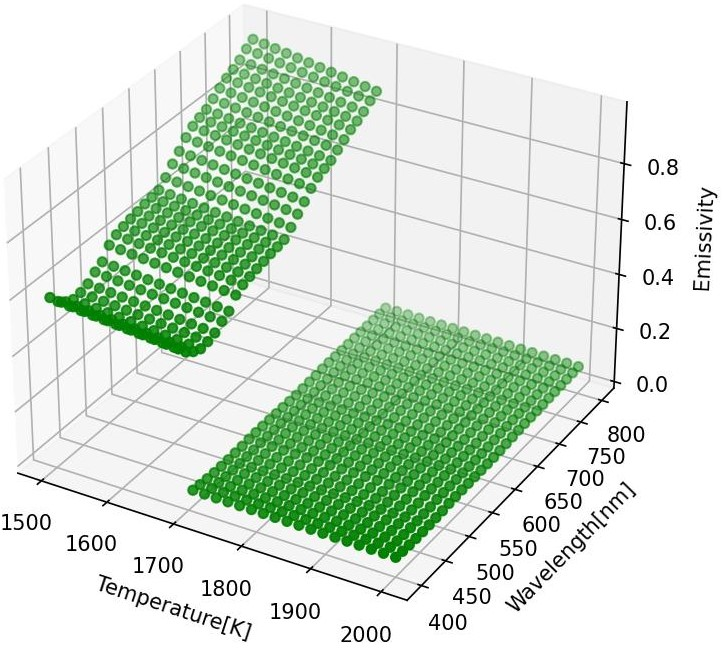
\includegraphics[width=0.6\textwidth]{figures/emissivity_model.jpg}
  \caption{Emissivity value along wavelength and temperature calculated from model 9}
  \label{fig: emissivity_model}
\end{figure}


Fig.\ref{fig: emissivity_model} shows the emissivity model based 
on model 9 in different temperature 
and wavelength. It can be found that the emissivity at a temperature 
below melting temperature ($1700K$) varies significantly with wavelength.
This is caused due to the raw emissivity data. Then, at liquid phase of 
the hypothetical material, emissivity decreases to a value lower than $0.1$.


Thus, the phase change phenomenon of hypothetical material is also characterized, 
which gives the virtual experiment platform more potential to simulate 
real experiments.


\subsection{Camera model}
After obtaining the temperature field and emissivity model of hypothetical material, 
the physical value of spectral radiation intensity should be calculated, then, 
the physical value of spectral radiation intensity is converted to 
digital value using camera model, which is the output of the complete virtual 
experiment platform. 


To ensure consistency and scalability within the program for future feature 
additions, all calculations in the program are conducted using metric units. 
For instance, temperature is measured in Kelvin, and wavelength is measured in 
meters. Therefore, it is crucial to note that the unit of wavelength in the camera 
model's calculations is meters, not nanometers. This ensures dimensional 
correctness throughout the integration process.


As mentioned in Fig.\ref{fig: received}, the camera model is based on an integration 
method, which integrate the spectral intensity received by the sensor along the 
specific range of wavelength. However, due to the varying quantum 
efficiency of each channel in sensor, it means that for a virtual camera 
with 8 channels, each pixel requires 8 independent integration operations. 
This operation requires a large computational effort. So, in order to 
accelerate the generation speed and thus reduce the time cost of virtual 
experiment platform, a parallel computing strategy is introduced.


\begin{figure}[htbp]
  \centering
  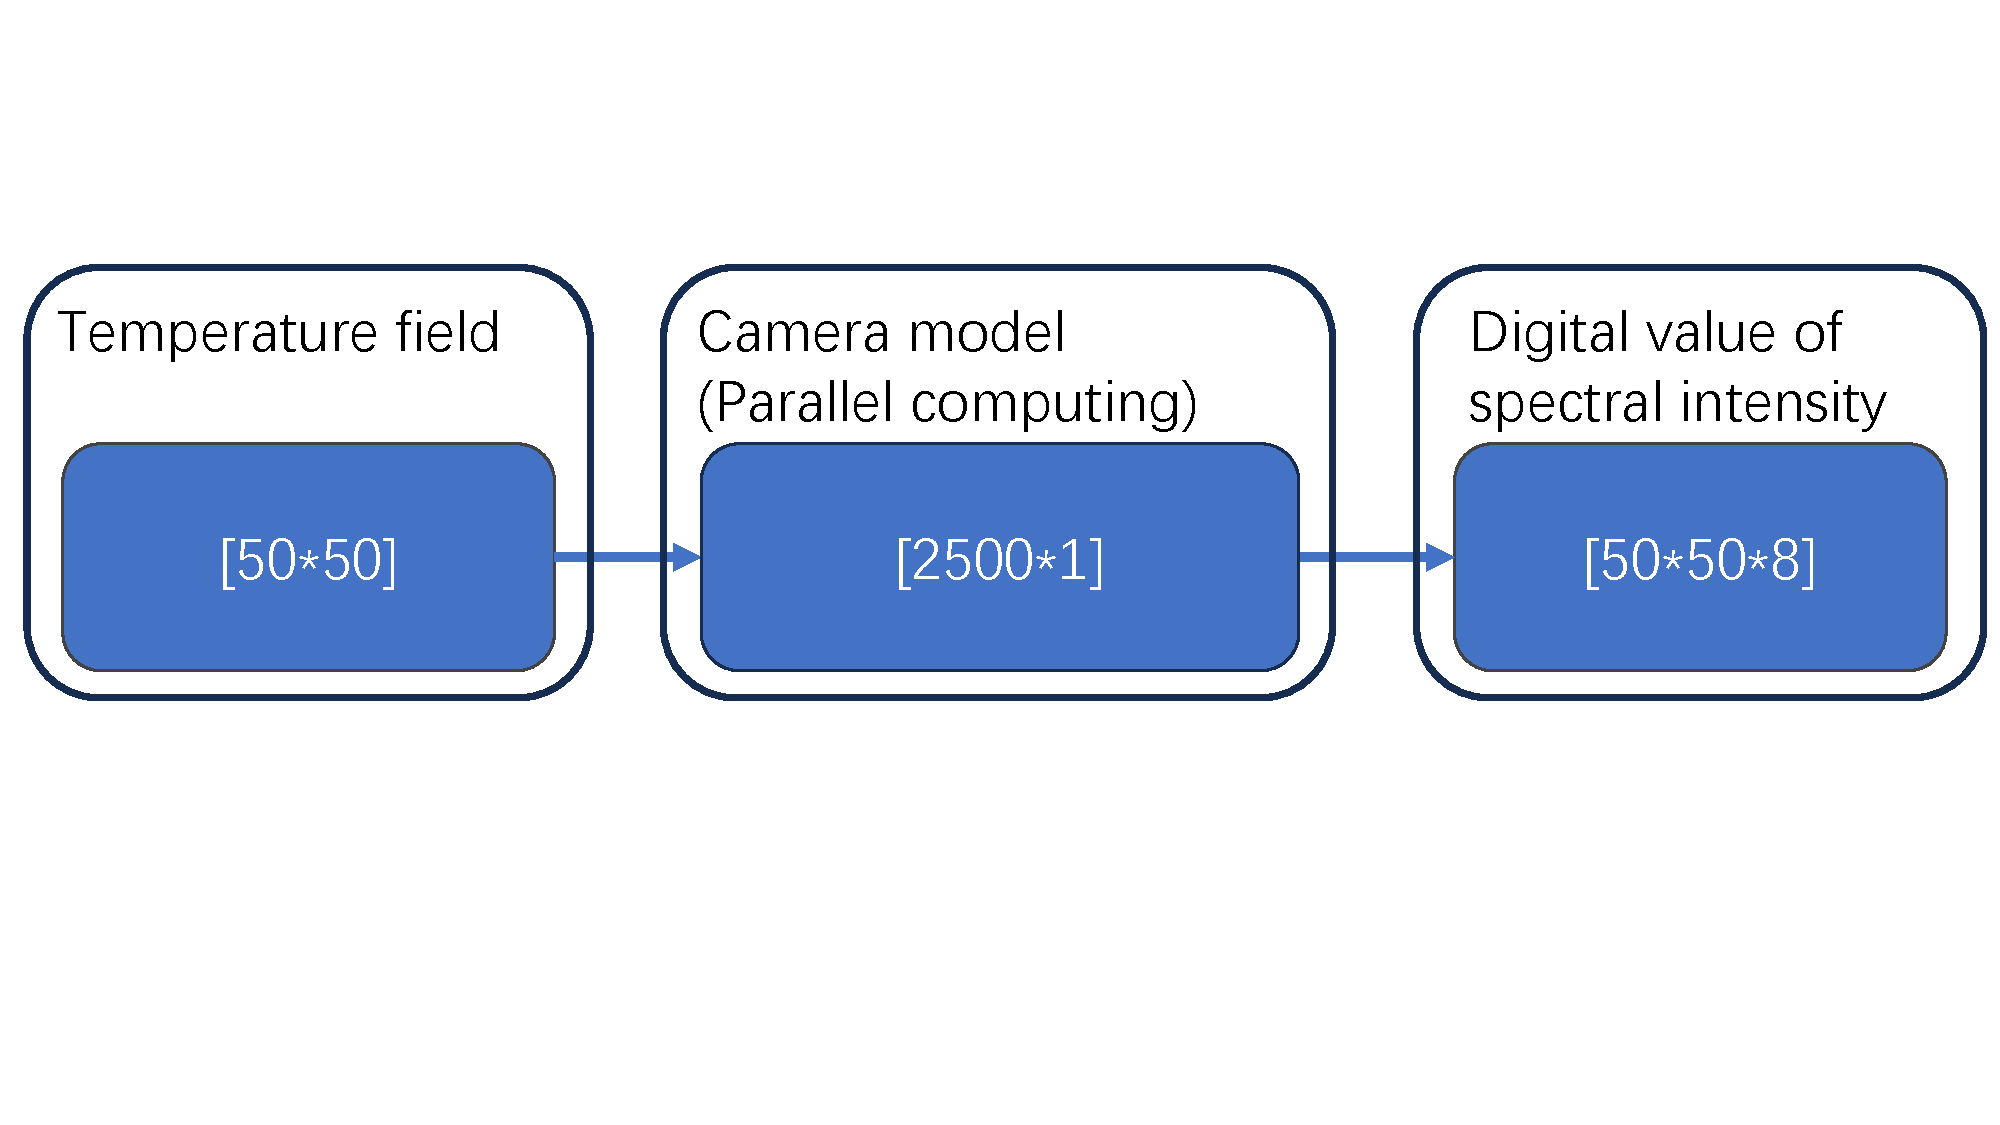
\includegraphics[width=0.9\textwidth]{figures/reshape.pdf}
  \label{fig: reshape}
  \caption{Shape of array used in camera model}
\end{figure}


The essence of parallel computing lies in decomposing a complex task into 
multiple tasks and utilizing multithreading techniques to execute these 
computational tasks simultaneously on different cores of the CPU. In 
this context, the camera model treats the integral computation on each pixel as an 
individual task, thereby significantly improving CPU utilization and substantially 
reducing computational time\cite{Asanovic.2009}. To facilitate task partitioning, the 
dimension of the temperature field 
mentioned earlier in this section needs to be reduced, from 
a $50\times 50$ matrix to a one-dimensional array of size $2500\times1$. This allows for 
obtaining 2500 parallel tasks. Once the calculations are completed, the 
resulting matrix of size $2500\times8$ is then transformed back into a three-dimensional 
matrix of size $50\times50\times8$. In this manner, a digital value similar to the data 
obtained in real experiments is computed.


\section{Temperature estimation algorithm}
After obtaining the digital value of spectral radiation intensity, 
the tasks of this virtual experiment platform are considered complete, 
and the next step involves data processing and calculations. The core 
of the temperature estimation algorithm lies in reconstructing the physical 
value of spectral radiation intensity based on the known digital values and 
the choosen parameters. 
Subsequently, through the implementation of a curve fitting algorithm, the 
estimated emissivity and temperature can be calculated.


\subsection{Rebuild physical value of spectral radiation intensity}
Hence, it is evident that the process of reconstructing the physical value holds 
significant importance in the temperature estimation algorithm. This reconstruction 
process represents the conversion of spectal radiation intensity from its physical value to a 
digital value. By analyzing the reconstructed results, the 
relationship between the physical value $(I_{rec})$ and the parameters $(T, k)$ to be fitted can be established, 
where $T$ and $k$ are derived from Eq.\ref{eq: reconstruct_integration}. Subsequently, 
by performing curve 
fit algorithm between the reconstructed physical value and the experimental data, we 
can obtain the parameters $(T, k)$ that best fit the real data. Therefore, it 
becomes apparent that the reconstruction of the physical value can affect 
the accuracy of the temperature prediction algorithm discussed in this thesis.


As mentioned in Eq.\ref{eq: reconstruct_integration}, the reconstructed physical value 
of spectral radiation intensity is generated based on the integration method. It can 
be observed that the digital value can be considered as a function of temperature of 
hypothetical material $T$ and parameters of emissivity model $k$.


\begin{equation}
  \label{eq: reconstruct_digital_value_function}
  I_{rec}^i (k, T) = q \int B(\lambda, T) \cdot \varepsilon(\lambda, k, T) 
  \cdot \eta_{camera}^i d\lambda
\end{equation}


Eq.\ref{eq: reconstruct_digital_value_function} shows the mathematical expression 
of reconstructed physical value of spectral radiation intensity of $i_{th}$ channel.
So, the current objective is to minimize the cost in Eq.\ref{eq: reconstruct_optimization} 
by optimizing the values of $k$ and $T$. In other words, the goal is to make the 
reconstructed spectral radiation intensity $I_{rec}(k, T)$ as close as possible 
to the values obtained in virtual experiments. By minimizing the cost function, 
the temperature estimation algorithm aims to achieve a high level of accuracy 
and fidelity in calculating the temperature based on the reconstructed 
digital values.


\subsection{Emissivity model used for calculation}
In the previous section, it is evident that the temperature estimation 
algorithm is essentially performing a curve fit algorithm on the parameters of the 
emissivity model and temperature of the hypothetical material. 
Therefore, the choice of the emissivity model significantly impacts 
the accuracy of the temperature estimation algorithm. In order to 
enhance the generality of this temperature prediction algorithm and 
prevent overfitting, a hypothesis is proposed: the temperature 
prediction algorithm is unaware of the material's emissivity 
characteristics. Hence, it is necessary to use a different 
emissivity model from the one used in the virtual experiment 
platform to reconstruct the digital value of spectral radiation 
intensity.


Based on mentioned above, the temperature estimation algorithm 
introduced in this paper tested several different emissivity 
models, namely:


\begin{enumerate}
  \item Linear model
  \item Linear square model
  \item Quadratic model
  \item Exponential model
  \item A combined model composed of the linear square and exponential models
\end{enumerate}


These models are distinguished based on the relationship between 
emissivity and wavelength. Each model represents a different 
mathematical expression that describes how emissivity varies with 
wavelength. In order to simplify the calculation process and thus set 
boundary conditions of parameters $k$ in emissivity model, all wavelength 
used in this emissivity model is normalized wavelength $\lambda_{norm}$. The 
mathematical expression can be described as followed:

\begin{equation}
  \label{eq: wavelength_norm}
  \lambda_{norm} = \frac{\lambda - \lambda_{lb}}{\lambda_{ub} - \lambda_{lb}}
\end{equation}


To enhance the readability of the formula, the parameter $k$ in 
Eq.\ref{eq: reconstruct_digital_value_function} is written in vector 
form in Eq.\ref{eq: k_vec} based on the number of parameters in emissivity model.

\begin{equation}
  \label{eq: k_vec}
  k = \begin{pmatrix}
    a \\
    b \\
    c \\
    \end{pmatrix} 
    or 
    \begin{pmatrix}
      a \\
      b \\
      \end{pmatrix}
\end{equation}
With the lower boundary of wavelength $\lambda_{lb} = 500 {nm}$ and the 
upper boundary of wavelength $\lambda_{ub} = 1000 {nm}$. Thus, the input 
of the emissivity model used in temperature estimation algorithm is thus 
dimensionless number.

\subsubsection{Linear model}
Linear model refers to a linear relationship between emissivity and wavelength,
which could be written as Eq.\ref{eq: emi_lin}:

\begin{equation}
  \label{eq: emi_lin}
  \varepsilon(\lambda) = a\cdot \lambda_{norm} + b
\end{equation}

The linear model represents the simplest and most straightforward emissivity model. 
It provides an easy way to visualize the calculated emissivity model 
and reduces complexity in defining various boundary conditions within the 
emissivity model.

\subsubsection{Linear square model}
The linear square model is distinct from the linear model, 
as it incorporates three parameters representing the coefficients 
of the quadratic term, the linear term, and the constant term. Its 
mathematical expression can be described as Eq.\ref{eq: emi_lin_square}:

\begin{equation}
  \label{eq: emi_lin_square}
  \varepsilon(\lambda) = a \cdot \lambda_{norm}^2 + b \cdot \lambda_{norm} + c
\end{equation}

The linear square model can be used to describe more intricate emissivity 
models for materials. With an additional parameter compared to the 
previous linear model, it offers increased degrees of freedom for 
curve fitting, enabling a better fit to complex shapes. Nevertheless, 
the augmented complexity may also lead to a higher risk of overfitting as 
well as increase of computational demand required.

\subsubsection{Quadratic model}
Consequently, in order to simplify the computation of the linear 
square model, the quadratic model was introduced. In this model, 
the coefficient of the linear term in the original linear square 
model is set to 0. This simplification leads to a reduction in 
the number of parameters within the emissivity model. The emissivity model 
can be expressed as Eq.\ref{eq: emi_quad}

\begin{equation}
  \label{eq: emi_quad}
  \varepsilon(\lambda) = a \cdot \lambda_{norm}^2 + b
\end{equation}

\subsubsection{Exponential model}
In the exponential model, emissivity is exponentially related to wavelength. Due to 
the monotonic nature of the exponential function, this model enhances the accuracy of 
parameter estimation along the gradient descent of the cost function during curve fitting, 
thereby improving the computational efficiency. The mathematical expression can be 
expressed in Eq.\ref{eq: emi_exp}:

\begin{equation}
  \label{eq: emi_exp}
  \varepsilon(\lambda) = \exp(-a \cdot \lambda_{norm} - b)
\end{equation}

For materrials commonly used in \gls{pbflbm}, emissivity tends to decrease with 
increasing wavelength. Therefore, to reduce the range of parameters during curve 
fitting, the exponent term $a \cdot \lambda_{norm} + b$ was set as non-negative value.

\subsubsection{Mixed model}
This model is a combination of two models. In Fig.\ref{fig: emissivity_model}, it 
can be observed that the emissivity of the virtual material undergoes 
significant changes when the temperature exceeds the material's melting point, 
and the emissivity variations become smaller in the liquid phase. Therefore, when 
emissivity changes are relatively small, i.e., when the material is in the 
liquid phase, the exponential model is more suitable. On the other hand, when 
emissivity changes are more pronounced, i.e., when the material is in the solid 
phase, the linear square model is more appropriate. This approach not only 
improves the computational accuracy of the model in the solid region but also 
ensures the computational efficiency of the model in the liquid region.


In this model, the computation starts with the linear square model. The computed 
results are then filtered to identify points where the temperature exceeds 
the material's melting point. Subsequently, the exponential model is 
utilized to recompute the emissivity and temperature for those specific points. 
Finally, the results from both calculations are combined to obtain a higher 
precision outcome. However, this process demands higher computational resources. 
Consequently, it is observed that this model significantly increases the 
computational time required for temperature estimation algorithms.


\subsection{Curve fit algorithm}
After obtaining the reconstructed physical values of intensity, 
a curve fit algorithm is required to determine  
temperature and the parameters of the emissivity model that best 
align with the actual received intensity. However, in this work, both 
the data obtained from the virtual experimental platform and the data 
from real experiments are not continuous spectral intensities. 
Conversely, the input for this temperature estimation algorithm is a 
two-dimensional array with dimensions of 8x2, which can be regarded as 8 
samples of a continuous physical value.


\begin{figure}[htbp]
  \centering
  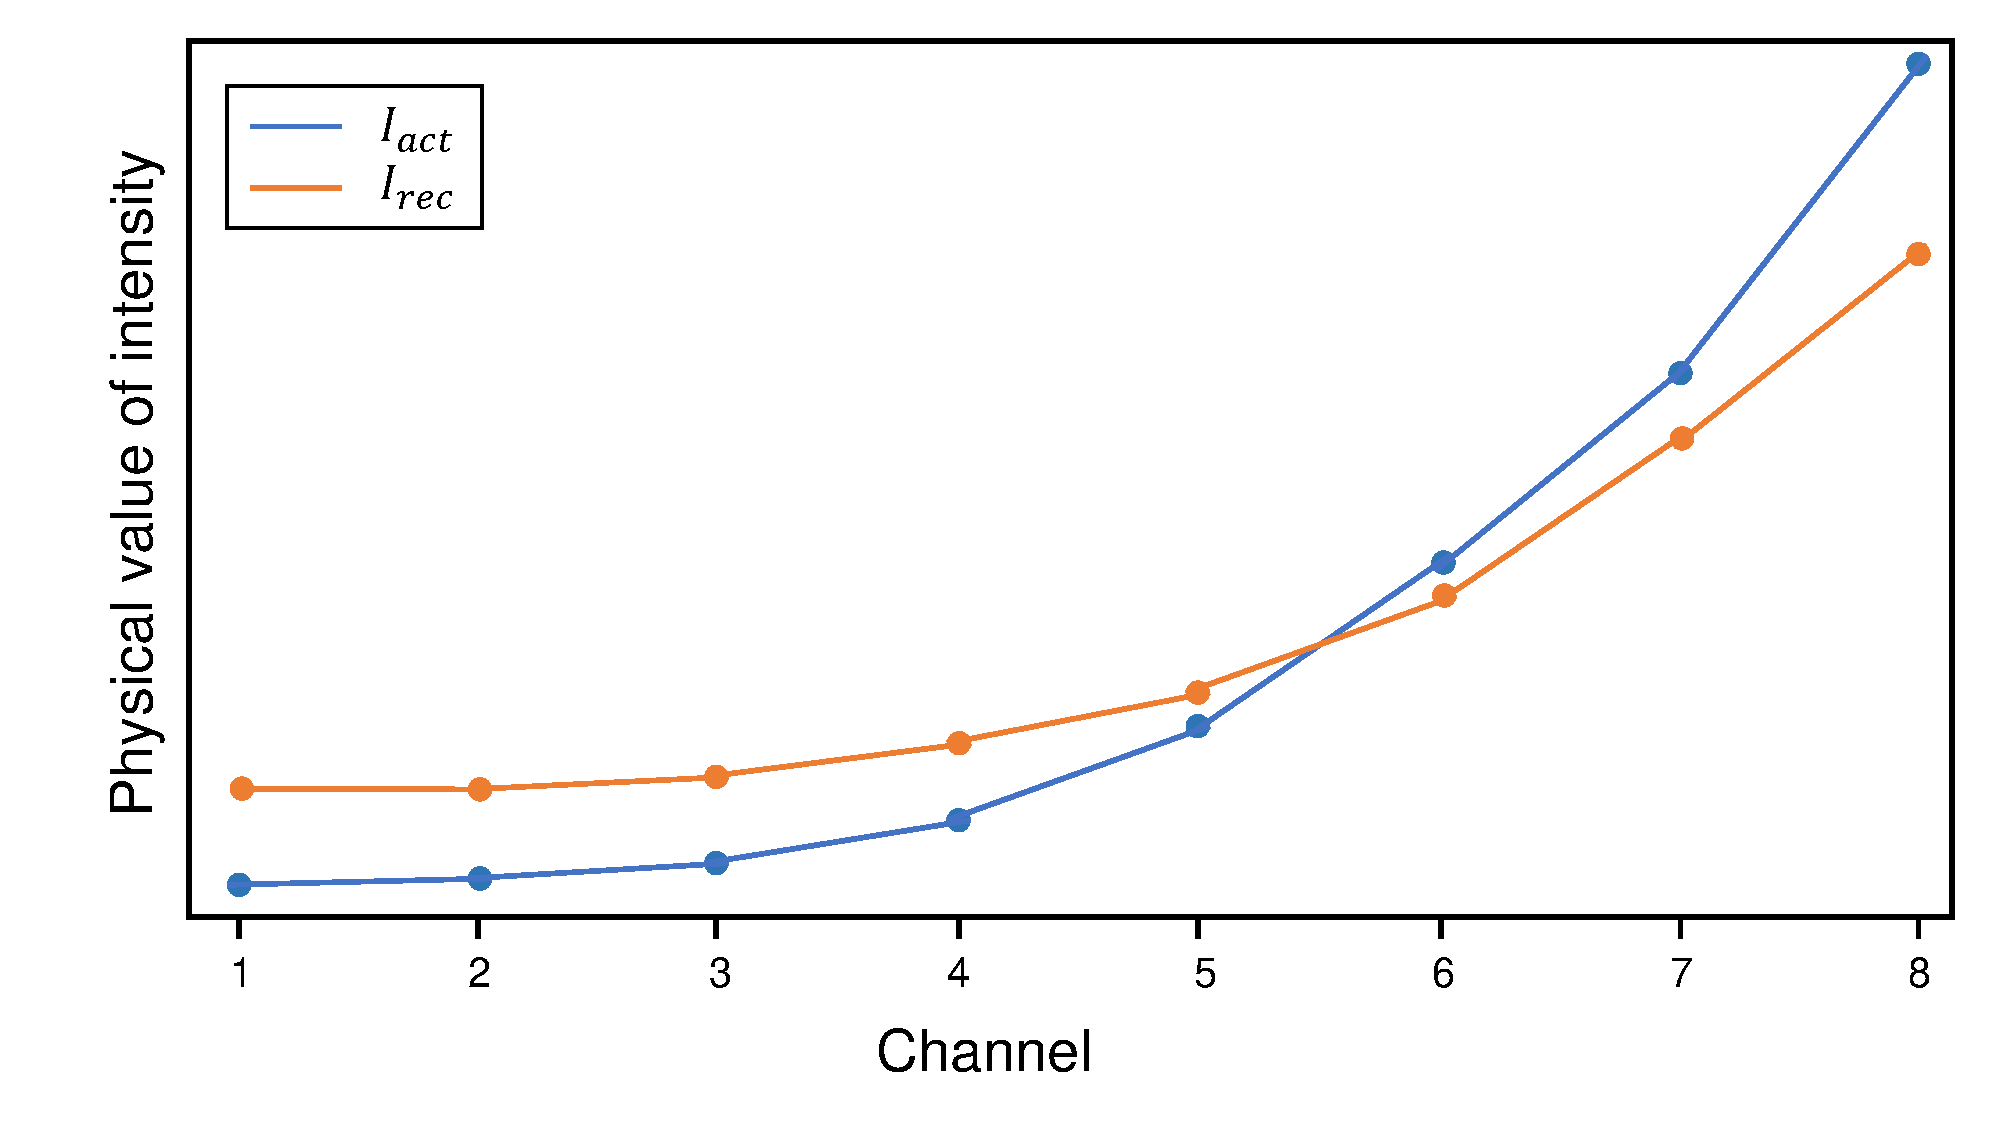
\includegraphics[width=0.9\textwidth]{figures/curve_fit.pdf}
  \caption{Comparison between actual received intensity $I_{act}$ 
  and reconstructed intensity $I_{rec}$ of one point}
  \label{fig: curve_fit_demo}
\end{figure}


Fig.\ref{fig: curve_fit_demo} illustrates the reconstructed physical 
value for each channel and the corresponding physical values from the 
original experimental data. It is evident that this approach simplifies 
the visualization of independent channel data and facilitates the 
utilization of this profile for curve fitting purposes.


\subsection{Parameters in temperature estimation algorithm}
The temperature estimation algorithm uses numerous parameters, 
which significantly impact the precision and consistency of the 
computed results. Therefore, it is essential to set boundary conditions 
for these parameters.


\subsubsection{Wavelength range}
In Fig.\ref{fig: quantum_efficiency}, it can be observed that the 
total quantum efficiency of the sensor $\eta_{camera}$ decreases to 
0 when the radiation wavelength exceeds 900 nanometers. This effect is 
attributed to the presence of a filter on the sensor. Consequently, 
when reconstructing the physical values of the spectral radiation 
intensity, the integration limits are set to be within the 
range of 500 nanometers to 1000 nanometers. This approach ensures 
that the essential information is captured while reducing the 
computational resources required for integration and thus improving the 
computational speed.


\subsubsection{Boundary condition of estimated temperature}
In the temperature estimation algorithm, the process starts with an 
initial guess, which is used to perform the first reconstruction of 
the physical values of the spectral radiation intensity. This 
reconstruction yields a cost function and a gradient that 
minimizes the cost function. The algorithm then adjusts the parameters 
to be optimized along this gradient before proceeding to the next 
iteration. It is evident that the choice of the initial guess 
significantly influences the computational efficiency of the 
program and can help avoid potential physically meaningless 
local minima.

To address this, it is mandated that the predicted temperature in the 
temperature estimation algorithm lie within the range of 500 to 2000K. 
This constraint ensures that the algorithm operates within a 
physically meaningful and relevant temperature range, preventing 
unrealistic results and potentially leading to a more effective and 
efficient optimization process.

\subsubsection{Boundary condition of estimated emissivity}
Unlike the boundary conditions applied to the estimated temperature, 
the boundaries for emissivity are much narrower. This is due to the 
physical definition of emissivity mentioned earlier in the text. 
Therefore, it is necessary to apply a boundary condition 
of $0 < \varepsilon < 1$ for emissivity during the calculations. 
However, in the curve fit algorithm mentioned in this work, emissivity 
is not a variable to be determined. Hence, it becomes necessary to 
incorporate this boundary condition directly into the emissivity model.